%% -*- LaTeX -*-
\documentclass{report}

\usepackage{thesis}

%some other packages I found useful, comment out or remove if you do not need them
\usepackage{amsmath}
\usepackage{amssymb}
\usepackage{amsthm}
\usepackage[titletoc,toc,title]{appendix}
\usepackage{chapterbib}
\usepackage{cite}
\usepackage [autostyle, english = american]{csquotes}
\usepackage{hyperref}
\usepackage[pdftex]{graphicx}
\usepackage{mathtools}
\usepackage{mdframed}
\usepackage{minted}
\usepackage{multirow}
\usepackage{newtx}
\usepackage{newunicodechar}
\usepackage{pdfcomment}
\usepackage{semantic}
\usepackage{subfigure}
\usepackage{tabularx}
\usepackage{textgreek}
\usepackage{titlesec}
\usepackage{url}
\usepackage{xspace}

% must be loaded after hyperref
\usepackage{cleveref}

\usemintedstyle{friendly}
%\setminted{fontfamily=lmtt}
\usepackage{zlmtt}
\usepackage[T1]{fontenc}

\newunicodechar{⇒}{\ensuremath{\Rightarrow}}
\newunicodechar{→}{\ensuremath{\rightarrow}}
\newunicodechar{λ}{\ifmmode\lambda\else\textlambda\fi}
\newunicodechar{Θ}{\ifmmode\Theta\else\textTheta\fi}
\newunicodechar{Γ}{\ifmmode\Gamma\else\textGamma\fi}
\newunicodechar{μ}{\ifmmode\mu\else\textmu\fi}
\newunicodechar{η}{\ifmmode\eta\else\texteta\fi}
\newunicodechar{Π}{\ifmmode\Pi\else\textPi\fi}
\newunicodechar{𐤄}{\ifmmode{\rotatebox[origin=c]{15}{\textphnc{e}}\hspace{-1pt}}\else{\textphnc{e}}\fi}
\newunicodechar{⊥}{\ensuremath{\bot}}
\newunicodechar{×}{\ensuremath{\times}}
\newunicodechar{⊳}{\ensuremath{\rhd}}
\newunicodechar{∩}{\ensuremath{\cap}}
\newunicodechar{∪}{\ensuremath{\cup}}
\newunicodechar{≠}{\ensuremath{\neq}}
\newunicodechar{∅}{\ensuremath{\varnothing}}
\newunicodechar{⊢}{\ensuremath{\vdash}}
\newunicodechar{△}{\ensuremath{\bigtriangleup}}
\newunicodechar{≡}{\equiv}
\newunicodechar{≢}{\not\equiv}
\newunicodechar{≤}{\ensuremath\leq}
\newunicodechar{⊕}{\oplus}
\newunicodechar{⊖}{\ominus}
\newunicodechar{⟦}{\lBrack}
\newunicodechar{⟧}{\rBrack}
\newunicodechar{∖}{\setminus}

\definecolor{myBGblue}{rgb}{0.94, 0.97, 1.0}

\newcommand{\BNF}{\quad\operatorname{::=}\quad}
\newcommand{\BNFOR}{\quad\operatorname{\big{|}}\quad}
\newcommand{\CASE}[6]{\langword{case}_{#1}#2\langword{of}\INL #3 ⇒ #4 ; \INR #5 ⇒ #6}
\newcommand{\CASEm}[6]{\begin{aligned}[t]\langword{case}_{#1}#2\langword{of}&\INL #3 ⇒ #4 ;\\& \INR #5 ⇒ #6\end{aligned}}
\newcommand{\COMM}[2]{\langword{com}_{#1;#2}}
\newcommand{\cmark}{\ding{51}}%
\newcommand{\DEF}{{\quad\operatorname{\triangleq}\quad}}
\newcommand{\DEFCASE}{\quad\operatorname{\xRightarrow{△}}\quad}
\newcommand{\DOT}{\langword{.}}
\newcommand{\eg}{\textit{e.g.}\xspace}
\newcommand{\FLR}[1]{\left\lfloor{#1}\right\rfloor}
\newcommand{\FST}[1]{\langword{fst}_{#1}}
\newcommand{\FuncLang}[1][small]{$𐤄_{λ\mathrm{#1}}$\xspace}
\newcommand{\ie}{\textit{i.e.}\xspace}
\newcommand{\INL}{\langword{Inl}}
\newcommand{\inlinecode}[2][haskell]{\mintinline[breaklines,bgcolor=myBGblue,fontsize=\small]{#1}{#2}}
\newcommand{\INR}{\langword{Inr}}
\newcommand{\langword}[1]{\operatorname{\mathsf{#1}}}
\newcommand{\LOOKUP}[2]{\langword{lookup}^{#1}_{#2}}
\newcommand{\mask}{\ifmmode{\operatorname{⊳}}\else{⊳}\fi\xspace}
\newcommand{\myference}[3]{\inference[\textsc{#1}]{#2}{#3}}
\newcommand{\netstep}[2]{\xlongrightarrow{ #1 \ifthenelse{\equal{#1}{}}{}{:} #2 }}
\newcommand{\nonempty}[1]{{#1^{+}}}
\newcommand{\noop}[2]{\mathtt{noop}^{\mask #1}\!\!(#2)}
\newcommand{\PAIR}{\langword{Pair}}
\newcommand{\prcstep}[2]{\xlongrightarrow{ ⊕#1 ; ⊖#2 }}
\newcommand{\RECV}[1]{\langword{recv}_{#1}}
\newcommand{\roles}[1]{\mathtt{roles}(#1)}
\newcommand{\SEND}[1]{\langword{send}_{#1}}
\newcommand{\set}[1]{\left\{#1\right\}}
\newcommand{\SND}[1]{\langword{snd}_{#1}}
\newcommand{\step}{\operatorname{\longrightarrow}}
\newcommand{\stepname}[1]{$\mathfrak{#1}$}
\newcommand{\vdbl}{\\[8pt]}
\newcommand{\xmark}{{\large $\times$}}%

\newcommand{\ChoreographyTS}{ChoreoTS\xspace}
\newcommand{\chorLambda}{Chor$\lambda$\xspace}
\newcommand{\Chorus}{ChoRus\xspace}
\newcommand{\dotcho}{\textsc{\textbf{.}CHO}\xspace}
\newcommand{\dtsim}{\textsc{DT-SIM}\xspace}
\newcommand{\HasChor}{Has\-Chor\xspace}
\newcommand{\HLSCentral}{$\boldsymbol{\lambda}_{\boldsymbol{C}}$\xspace}
\newcommand{\HLSLocal}{$\boldsymbol{\lambda}_{\boldsymbol{L}}$\xspace}
\newcommand{\HLSNet}{$\boldsymbol{\lambda}_{\boldsymbol{N}}$\xspace}
\newcommand{\minichor}{Mini\-Chor\xspace}
\newcommand{\MultiChor}{Multi\-Chor\xspace}

\newtheorem{theorem}{Theorem}
\newtheorem{lemma}{Lemma}
\newtheorem{corollary}{Corollary}

\newtheorem*{future}{Future Work}

%\newcommand{\todo}[1]
%    {{\color{red} \fbox{\bfseries\sffamily\scriptsize{TODO}}
%    {\small$\blacktriangleright$\textsf{\emph{#1}}$\blacktriangleleft$}}~}

\widowpenalty=1000000
\clubpenalty=1000000

\MakeOuterQuote{"}


\title{A New Architecture for\\Choreographic Programming Languages}
\author{Mako Bates}
\defendingOn{2025}{June}{27}
\graduatingIn{2025}{August}
%\proposal % or finalpresentation
\finalpresentation
\dissertation                             %% or \dissertation
\doctorphilosophy                      %% or \doctorphilosophy or \masterarts
\cs                                 %% this is the only speciality defined.
\advisor{Joseph P. Near, Ph.D.}
\readerone{Christian Skalka, Ph.D.}
\readertwo{Yuanyuan Feng, Ph.D.}      %% Optional if MS.
\readerthree{Andrew K. Hirsch, Ph.D.}
\chair{Alice Patania, Ph.D.}
\dean{Holger Hoock, DPhil}


\begin{document}
\maketitle


\begin{abstract}
  Choreographic programming (CP) is a paradigm for implementing
  distributed systems that uses a single global program to define the
  actions and interactions of all participants.
  One characteristic of CP is that values are "located",
  \ie associated or annotated with parties who own them,
  and non-owners of a located value cannot use it.
  %
  Existing CP systems are generally either \emph{select-\&-merge} systems,
  which have a designated "select" operator for communicating knowledge of choice,
  or use alternative strategies that are known to be less efficient.
  
  We make four contributions to the ongoing development of CP systems.
  First, we propose and formalize \emph{conclaves} and \emph{multiply-located values};
  this combination of features enables efficient conditionals
  without redundant communication or a specialized operator.
  Second, we implement this "conclaves-\&-MLVs" paradigm in Haskell as the \MultiChor library.
  Third, we propose
  \emph{census polymorphism}, a technique for abstracting over the
  number of participants in a choreography.
  Forth, we demonstrate the viability of a CP system \minichor that uses only conclaves and has no designated syntax for located values.

  \MultiChor is available to end-users now,
  and contains solutions to key engineering problems.
  Based on anecdotal experiences using it
  and subsequent work on the theory-oriented fork \minichor,
  we outline near-term avenues for future work on CP systems for industry use.
\end{abstract}

\begin{citationspage}
\citationheadingpublished

\noindent Bates, M. and Kashiwa, S. and Jafri, S. and Shen, G. and Kuper, L. and Near, J. P..
	  (2025). Efficient, Portable, Census-Polymorphic Choreographic Programming. {\it PLDI25}.
\end{citationspage}

\tableofcontents
\listoffigures
%\listoftables

\mainmatter
\sloppy

%for journal format dissertation each chapter needs its own reference section, and want references to be included in global bibliography
%this is accomplished using include commands
%but, for things like the lit review (chapter 1) or an appendix, should use input so it does not get it's own references section

%if not doing a journal format dissertation you can just use input for all chapters, or put text here directly.
\chapter{Introduction and Literature Review}

\begin{quote}
Choreographic programming is a language paradigm for writing concurrent software systems of various kinds.
It's comparatively young; while some of the ideas have existed informally as far back as the 1970s,
choreographic programming as it's understood today was first formalized in~\shortcite{montesi-carbone-dfbd}.
In this chapter we describe the central concepts of choreographic programming,
its advantages and disadvantages,
and past and ongoing work to push the boundaries of the kinds of systems it can implement.
\end{quote}

\section{Introduction}

Choreographic programming (CP)
is a paradigm for implementing distributed systems in which the programmer writes one unified program, called a choreography,
that describes how the participants of the system interact
from a third-person-omniscient perspective.~\shortcite{montesi-carbone-dfbd,montesi-dissertation,montesi_book}
A choreography can be translated into to a collection of executable programs for use in the real world, one for each participant;
this process is called endpoint projection (EPP).
The CP approach has benefits both for understandability of distributed system implementations,
and for strong static guarantees about the deadlock-freedom of the resulting executable code~\cite{montesi-carbone-dfbd}.

\subsection{An illustrative example}

Consider the three programs in \Cref{fig:kvspiecewise},
which are intended to run concurrently and pass messages back and forth between each other.
The overall effect is an elementary process in which the client makes a \inlinecode{Get} or \inlinecode{Put} request to
a server (with a backup) that manages a key-value-store (KVS).
Even this simplified example takes a moment for a reader to make sense of;
one must read the three programs, infer the correspondence between messages sent and received by the three parties,
and judge for oneself if the communication protocol implemented is sensical.
One might even judge that this simple protocol has a bug:
if the request is a \inlinecode{Get}, the backup server will hang indefinitely!

\begin{figure}[tbhp]\caption{A Simple Concurrent Protocol: a key-value store with a backup server}
  \begin{mdframed}
  \begin{tabular}{c}
  \begin{minipage}{12.5cm}
    \inputminted[xleftmargin=10pt,linenos,fontsize=\scriptsize]{haskell}{figures/kvs_piecewise_client.hs.txt}
  \end{minipage} \\\\
  \begin{minipage}{12.5cm}
	  \textbf{(a)} The function to be called by the client process.
	  They pass in their \inlinecode{Request} object and send it to the server.
	  Then they receive a response from the server and return it.
  \end{minipage}\\\\
  \hline\\
  \begin{minipage}{12.5cm}
    \inputminted[xleftmargin=10pt,linenos,fontsize=\scriptsize]{haskell}{figures/kvs_piecewise_server.hs.txt}
  \end{minipage} \\\\
  \begin{minipage}{12.5cm}
  The function to be called by the primary server.
	  They pass in a reference to their mutable state, and receive a message of type \inlinecode{Request} from the client.
	  In the case of a \inlinecode{Put} request, they forward it to the backup server and check for the backup's acknowledgement.
	  In either case, they process the request against their own mutable state and send the response back to the client.
  \end{minipage}\\\\
  \hline\\
  \begin{minipage}{12.5cm}
    \inputminted[xleftmargin=10pt,linenos,fontsize=\scriptsize]{haskell}{figures/kvs_piecewise_backup.hs.txt}
  \end{minipage} \\\\
  \begin{minipage}{12.5cm}
  The function to be called by the backup server.
	  They pass in a reference to their mutable state, and receive a \inlinecode{Put} message from the primary server.
	  They process it against their mutable state and send back an acknowledgement message to indicate their success.
  \end{minipage}
  \end{tabular}
  \label{fig:kvspiecewise}
  \end{mdframed}
\end{figure}

In \Cref{sec:background} we will mention some intermediate frameworks that have historically been used to facilitate
writing large and complicated concurrent protocols,
but here we jump ahead to choreographic programming (CP).
\Cref{fig:kvspseudo} shows the same protocol as \Cref{fig:kvspiecewise}, but implemented as a choreography.
In this form there is no cognitive overhead for matching \inlinecode{send} and \inlinecode{recv} operations,
because matching pairs of them are combined into monolithic \inlinecode{comm} operations.
The entire protocol can be read at once in a sensical order.
(The order in which operations are presented in a choreography is not necessarily the order in which they will happen;
the participants are not guaranteed to all start at the same physical time, or to operate at the same speeds.)
Re-writing the example KVS system as a choreography does not immediately solve the issue
of what the backup server should do in the event of a \inlinecode{Get} request,
but it makes the problem detectable by static analysis.
In fact, the choreography in \Cref{fig:kvspseudo} cannot compile in any real CP system
because \inlinecode{"backup"}'s behavior is ambiguous.
\Cref{fig:kvsenclave} shows two variations of how to realize the KVS behavior in Haskell using our \MultiChor library.

\begin{figure}[tbhp]\caption{A Simple Choreography: a key-value store with a backup server}
  \begin{mdframed}
  \begin{tabular}{c}
  \begin{minipage}{12.5cm}
    \inputminted[xleftmargin=10pt,linenos,fontsize=\scriptsize]{haskell}{figures/kvs_pseudo.hs.txt}
  \end{minipage} \\\\
  \begin{minipage}{12.5cm}
	  A pseudo-code choreographic implementation of the protocol from \Cref{fig:kvspiecewise}.
  \end{minipage}
  \end{tabular}
  \label{fig:kvspseudo}
  \end{mdframed}
\end{figure}


\begin{figure}[tbhp]\caption{A Real Choreography: a key-value store writing using \MultiChor}
  \begin{mdframed}
  \begin{tabular}{c c}
  \begin{minipage}{8.75cm}
    \inputminted[xleftmargin=10pt,linenos,fontsize=\scriptsize]{haskell}{figures/kvsenclave_a.hs.txt}
  \end{minipage}
  &
  \begin{minipage}{3.75cm}
    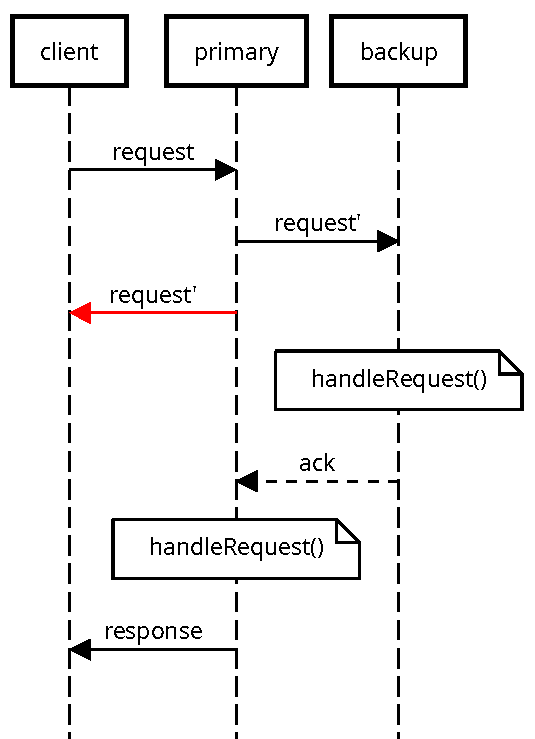
\includegraphics[width=4cm]{figures/seq2.pdf}
  \end{minipage} \\\\
  \multicolumn{2}{c}{\begin{minipage}{12.5cm}
  A key-value store with a backup server, written in \MultiChor.
           The backup server sends an acknowledgement message \textsf{ack} to the primary server
           if and only if \inlinecode{request} is a \inlinecode{Put}.
           The \inlinecode{broadcast} operator (line 19) ensures KoC
           so that the primary and backup servers are guaranteed to use the same case of \inlinecode{handleBackup},
           but it results in redundant communication (shown in red in the sequence diagram).
  \end{minipage}}\\\\
  \hline\\
  \begin{minipage}{8.75cm}
    \inputminted[xleftmargin=10pt,linenos,fontsize=\scriptsize]{haskell}{figures/kvsenclave_b.hs.txt}
  \end{minipage}
  &
  \begin{minipage}{3.75cm}
     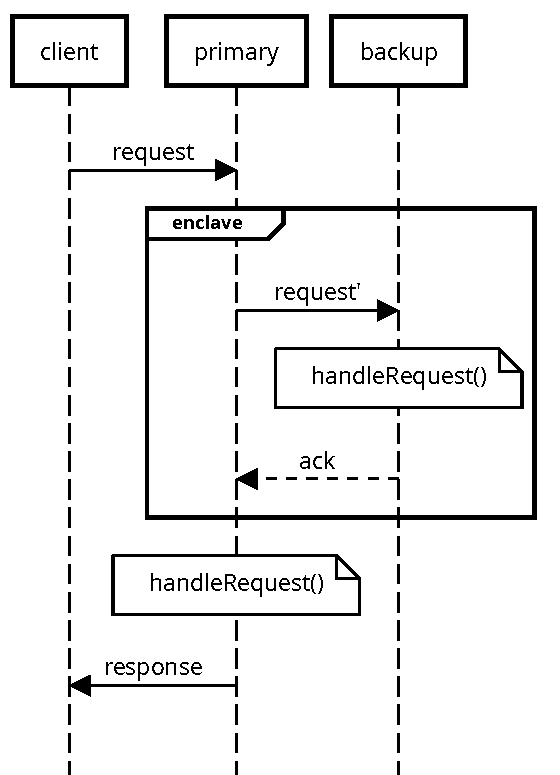
\includegraphics[width=4cm]{figures/seq3.pdf}
  \end{minipage} \\\\
  \multicolumn{2}{c}{\begin{minipage}{12.5cm}
  In this variation, the \inlinecode{enclave} operator eliminates the redundant communication.
           The enclaved sub-choreography is indicated by a box in the sequence diagram.
           On line~2, \inlinecode{@@ nobody} is \MultiChor idiom explained in \Cref{sec:membership}.
  \end{minipage}}
  \end{tabular}
  \label{fig:kvsenclave}
    %%\Description{In the top section, twenty four lines of Haskell code using the MultiChor library, with a UML sequence diagram of that program.
%%	The code defines a choreography called "kvs", and helper-functions "handleRequest" and "handleBackup".
%%	In the sequence diagram, first "client" sends "request" to "server",
%%	  then "server" sends "request-prime" to "client" and "backup",
%%	  then backup calls "handleRequest",
%%	  then backup may send "ack" to "server",
%%	  then server calls "handleRequest",
%%	  then server sends "response" to "client.
%%	The bottom sections shows changes to the code in the top section.
%%	In particular, the return type of "handleBackup" is changed to exclude "client".
%%	In the updated sequence diagram, the part of the protocol representing "handleBackup" is in a box named "enclave",
%%	  and the spurious transmission of "request-prime" from "server" to "client" is omitted.
%%	  }
  \end{mdframed}
\end{figure}


Here is a citation, \shortcite{li2021model}.

\subsection{Layout and Contributions}

The remainder of this chapter covers the history and theory of CP
and discusses some modern work relevant to the ongoing development of CP systems.
In particular, \Cref{sec:knowledge-of-choice} discusses the "Knowledge of Choice" problem,
a central difficulty in the design of CP systems,
and a number of strategies that have been used to solve it.

\Cref{sec:formalism} presents our first contribution:
a formal model of a CP system with two novel features:
\emph{multiply-located values} (MLVs)
and \emph{enclaves}.
These features combine to allow a compelling new strategy for KoC management.
In particular, all well-typed \HLSCentral choreographies are projectable and have cromulent KoC by construction.
In \Cref{sec:formalism-comparisons} we compare \HLSCentral to representative systems that use other KoC management strategies.

\Cref{sec:multichor} presents our second contribution: an implementation of the enclaves-\&-MLVs paradigm in Haskell.
The \MultiChor library is already available on Hackage, Haskell's main package management system.
\MultiChor directly implements the main concepts of \HLSCentral as a monadic eDSL in Haskell,
and combines Haskell's Hindley–Milner-based type system with a proof-witness system
to capture the requisite notion of a well-typed choreography.

Because \MultiChor is fully embedded in and interoperable with Haskell,
functional-programming patterns can be applied to the choreographic setting without further theoretical or infrastructural work.
The most important example of this, which we call "census polymorphism" is the ability to write choreographies
that are parametric over their set of participants.
This capability is novel among CP systems, and the third contribution presented in this work.
We discuss census polymorphism in greater detail in \Cref{sec:census-poly}.
\Cref{sec:future-implementation} reviews some promising future, both theoretical and at the engineering level,
that could improve \MultiChor's utility.



\section{Background}
\label{sec:background}
In this section, we give a brief overview of choreographic programming (CP).
For a comprehensive introduction to the topic, we refer the reader to~\cite{montesi_book}.

Choreographic programming is a paradigm that expresses a distributed system
as a single, global program describing the behavior and interactions of all parties.
The global view of the distributed system enables easier reasoning about the system's behavior;
for example choreographic languages can ensure \emph{deadlock freedom}~\cite{montesi-carbone-dfbd}
and choreographies can be composed modularly like normal single-threaded protocols.



\subsection{Knowledge of Choice}
\label{sec:knowledge-of-choice}

Choreographies with conditionals
(\inlinecode{if}-expressions or anything that could be used for conditional control-flow)
introduce
a challenge for endpoint projection:
\emph{some parties might not know which branch to take!}
This challenge is referred to as the \emph{knowledge of choice}  (KoC)~\cite{castagna-knowledge-of-choice} problem.
All choreographic programming languages include a strategy for KoC
that ensures that relevant parties have enough information to play their part in the program.

\subsection{Endpoint Projection}
\label{sec:endpoint-projection}
Maybe this goes before KoC; I haven't decided.

\subsection{The "Census" typing context}
\label{sec:census}
Although it is a hallmark of CP that a user may write actions for various parties in any given place in the program
without demarcations of who "control" is passing to,
it is not necessarily the case that every party that exists is eligible to take action at every place in the choreography.
Some earlier works, \eg \cite{chor-lambda}, have tracked these sets of participants in their type systems,
and used that typing context to control participation inside of function bodes.
Such a typing context plays a more active role in this present work, so we coin the term \emph{"census"}
for a typing context that controls which parties are "present" to participate in any given part of a choreography.

A party not listed in a census should will typically skip evaluating that section of the choreography.
In terms of EPP, that's done by projecting the entire clause to ⊥ or some similar marker.

\subsection{Additional Literature}
\label{sec:modern-work}

Review recent work on CP systems, including other systems that use MLVs.


\bibliographystyle{chicago}
\bibliography{refs}

\chapter{A New Core Choreographic Calculus}
\chaptermark{Formalism???} %this is the chapter heading that will show on subsequent pages
\label{sec:formalism}

\begin{quote}
Do chapters really need their own abstracts?
\end{quote}


\section{Introduction}
Plan A is to copy-paste large sections of \emph{"We Know I Know You Know"}, with revisions from the enclaves paper etc as needed.
Iff I make a new formalism, then I'll have to decide how to integrate it here. 

\section{Comparisons with other systems}
\label{sec:formalism-comparisons}
In particular, how does E\&M stack up against S\&M?
This could also just be copy-pasta, or we could expand it with something more like a proof.

A citation might help this compile? \shortcite{shen-alg-eff-cp}

\bibliographystyle{chicago}
\bibliography{refs}

\chapter{Real World Choreographic Programming}
\chaptermark{\MultiChor: Real World Choreographic Programming} %this is the chapter heading that will show on subsequent pages
\label{sec:multichor}




\section{Introduction}
In this chapter we demonstrate the practicality of conclaves-\&-MLVs choreographic programming
by presenting our implementation:
the \MultiChor Haskell library.
\MultiChor is a "just a library" CP system in the style of HasChor.
We adopt HasChor's freer-monads and handlers design pattern,
and embed the key aspects of \HLSCentral's type system as type-level constraints with a bespoke proof-witness system.
Furthermore, the flexibility of \MultiChor's API and the power of Haskell's type system together suffice to support \emph{census polymorphism},
a novel capability in CP systems.

A key innovation of \HLSCentral is that KoC is enforced entirely
by type-level management of the census.
By representing the census as a type-level variable in Haskell,
\MultiChor enables polymorphism over both the size and membership of the census,
a feature not considered in the construction of \HLSCentral.
All Haskell typing happens statically, and \MultiChor's EPP happens at runtime (like HasChor's).
This means that, like other cases of polymorphism in Haskell, location polymorphism in \MultiChor must be resolved statically.

A few other desiderata motivate our implementation:
\begin{enumerate}
    \item It should be possible to broadcast, \ie to multicast a value to the entire census,
          and to use values known to the entire census as normal (un-located) values of their type.
    \item It should be possible to know from an appropriately-written choreography's type that some
          certain party or parties are not involved, are not in its census.
          Users should be able to embed such "conclave" choreographies inside choreographies with larger,
          possibly polymorphic, censuses.
    \item The type system should be able to reason about parties'
          membership in a census or ownership-set
          with normal subset reasoning.
\end{enumerate}
The choreography in \Cref{fig:card-game} showcases the above points.
The census of the whole program appears in the type
and does not specify who the players are.
The \inlinecode{conclave} on line~16
embeds a choreography whose census is exactly the monomorphic \inlinecode{"dealer"}
and a polymorphic \inlinecode{player} (\#2).
The helper-function \inlinecode{broadcast} on line~18 functions as described in \#1.
Many examples of \#3 are automated or hidden in \MultiChor,
but on line~16 the function \inlinecode{inSuper} is applied to
\inlinecode{players :: Subset players ("dealer" : players)}
and \inlinecode{player :: Member player players}
to attest that \inlinecode{player} is present in the census.

\begin{figure*}[tbhp]
    \begin{mdframed}
  \begin{tabular}{c}
  \begin{minipage}{0.95\linewidth}
    \inputminted[xleftmargin=10pt,linenos,fontsize=\footnotesize]{haskell}{figures/census-poly-example.hs.txt}
  \end{minipage} \\\\
  \begin{minipage}{0.95\linewidth}
             This choreography is polymorphic over the number and identity of the players,
             but the party named \inlinecode{"dealer"} is an explicit member.
             The inner monad \inlinecode{CLI} that all parties have access to is a simple freer monad
             that can be handled to IO operations, or as \inlinecode{State} for testing purposes.
             The \inlinecode{newtype Card} encapsulates the modulo operation in its
             \inlinecode{Num} instance.
  \end{minipage}
  \end{tabular}
    \caption{A card game expressed as a choreography written in \MultiChor.}
    \label{fig:card-game}
    %\Description{Thirty lines of haskell code describing a choreography called "game".}
    \end{mdframed}
\end{figure*}


\section{Censuses, Conclaves, and MLVs in Haskell}
\label{sec:implementation}

\MultiChor uses the same free-monad approach as \HasChor~\cite{shen-haschor} to implement choreographic programming, EPP,
and the final interpretation to a real communication mechanism.
Also like \HasChor, \MultiChor's \inlinecode{Choreo} monad is parameterised by a \emph{local monad} in which parties' local computations can be expressed.
A \MultiChor type \inlinecode{Located ps t} is a multiply-located \inlinecode{t} owned by the parties \inlinecode{ps}.
It is possible to write \MultiChor functions that look and work like each of \HasChor's three primitive operators,
but the derived API in which users write \MultiChor choreographies contains a clear analog of only one of \HasChor's primitives.
Haskell's monadic-\inlinecode{do} notation and purity-oriented type system make \MultiChor code concise and safe
(in the sense that users are unlikely to accidentally invalidate important invariants).

As explained in \Cref{sec:formalism},
our KoC strategy requires that the correctness (well-typed-ness) of choreographies be judged in the context of a census.
\MultiChor adds the census as a type parameter of the \inlinecode{Choreo} monad.
Its kind is \inlinecode{[Symbol]},
which is to say that the census is a type-level list of parties and parties are type-level strings.
\inlinecode{Choreo} is \emph{not} an \emph{indexed} monad (that is, executing a monadic operation doesn't change the census),
but monadic operations can take choreographies with smaller censuses as arguments.

\begin{figure*}[tbhp]
  \begin{mdframed}
  \begin{tabular}{c}
  \begin{minipage}{0.95\linewidth}
    \inputminted[xleftmargin=10pt,linenos,fontsize=\footnotesize]{haskell}{figures/operators-multichor.hs.txt}
  \end{minipage} \\\\
  \begin{minipage}{0.95\linewidth}
        Of these four operators, \inlinecode{conclave} is the only one users will usually call directly;
        the other three can combine with each other (and with \inlinecode{conclave}) to make more user-friendly alternatives.
  \end{minipage}
  \end{tabular}
    \caption{
        The fundamental operators for writing expressions in \MultiChor's \inlinecode{Choreo} monad.
    }
    \label{fig:operators-multichor}
    %\Description{Four type signatures for Haskell functions using the MultiChor library.}
  \end{mdframed}
\end{figure*}

The fundamental operations of \MultiChor's \inlinecode{Choreo} monad are
\inlinecode{conclave}, \inlinecode{broadcast'}, \inlinecode{locally'}, and \inlinecode{congruently'}.
Their type signatures are given in \Cref{fig:operators-multichor}.
Like in \HasChor, these are free-monad constructors; their behavior is implemented in interpreters
that carry out EPP or implement a centralized semantics.
Three of them have their names "primed" because the un-primed versions of these names are reserved for more ergonomic derived functions.
For example, \inlinecode{locally'} takes a single argument, a computation in the local monad, and requires that the census contains
\emph{a single party}, who will execute that computation.
The un-primed \inlinecode{locally} takes an additional argument that identifies a single party from a larger census;
it uses \inlinecode{conclave} to correctly call \inlinecode{locally'}.
\inlinecode{broadcast} shares a \inlinecode{Located} value with the entire census so the unwrapped value can be used;
by combining this with \inlinecode{conclave} we can implement point-to-point or multicast communication.
From the perspective of a centralized semantics, \inlinecode{conclave} doesn't do anything at all besides run
the sub-choreography,
but EPP to a party \emph{not} in the sub-census skips the sub-choreography and just returns \inlinecode{Empty}.

\inlinecode{congruently} lets us leverage MLVs to concisely write actively-replicated computations.
In contrast to \inlinecode{locally}, the computation is performed by multiple parties
and the result is multiply-located across all of them.\footnote{
    The entire census participates in the primed version, and its result is returned naked.
    The behavior of \inlinecode{conclave} and the more fundamental rules of monadic programming
    ensure the un-primed \inlinecode{congruently} behaves correctly.
}
For the execution of these actively-replicated computations to correctly return an MLV,
all the parties must be guaranteed to be doing a pure computation on the same data.
Haskell makes it easy to enforce such a guarantee to a practical (but not unbreakable) extent.
This is why \inlinecode{congruently} does not grant access to the local monad \inlinecode{m}.
It also requires that the computation not have access to the specific identity of the computing party,
unlike \inlinecode{locally} and the similar-looking function \inlinecode{parallel} mentioned in \Cref{sec:census-poly}.
Weakening (or subverting) these restrictions would allow a user to violate \MultiChor's invariant that MLVs (\inlinecode{Located} values)
have the same value across all their owners.

It is critical to the safety of \MultiChor that the projection of a choreography to any given party will not use
any other party's \inlinecode{Located} values.
We use the same basic strategy for this as \HasChor:
\inlinecode{Located}'s constructors, \inlinecode{Wrap} and \inlinecode{Empty}, are hidden inside the core module
and afforded only by dependency injection to \inlinecode{locally} and \inlinecode{congruently}.
The specific "unwrapper" functions afforded to \inlinecode{locally} and \inlinecode{congruently}
are known to user code only by their type signatures, which have respective aliases \inlinecode{Unwrap} and \inlinecode{Unwraps}.
\inlinecode{Located}'s constructors are also used by two less-critical functions, \inlinecode{flatten} and \inlinecode{othersForget}.
These are needed for shrinking ownership sets or un-nesting \inlinecode{Located} values;
they could be written using \inlinecode{congruently},
but by implementing them in the core module where they can pattern-match \inlinecode{Located} values we are able to make them not-monadic,
and so more convenient.


\section{Membership Constraints \& Proof Witnesses}
\label{sec:membership}

It is not trivial for Haskell's type-checker (a component of GHC, the compiler) to judge if
a particular participant owns a multiply-located value or is present in a particular census
when the party or the set are polymorphic.
Declaring membership and subset relations as class constraints can work in some situations,
but this strategy has serious limitations which we find unacceptable.
For example, a rule as obvious as
$(p \in ps_1 \land ps1 \subseteq ps_2) \to p \in ps_2$,
represented in Haskell as
\inlinecode{instance ( IsMember p ps1, IsSubset ps1 ps2) => IsMember p ps2},
would be impossible to use because the compiler has no way of guessing which set \inlinecode{ps1}
it should be checking \inlinecode{p}'s membership in.
(Even if it could \emph{guess}, it wouldn't backtrack and try a different guess when its first try didn't work).

To work around such limitations, \MultiChor uses a strategy of \emph{proof witnesses}
like those described by \cite{noonanGDP}.
These are light-weight runtime values with specially crafted types,
such that the existence of a value of the given type guarantees the truth of some logical assertion.
We do not actually use the \inlinecode{gdp}\footnote{
    "Ghosts of Departed Proofs"~\cite{gdp_hackage}
} package; we found that writing our own purpose-specific system had a few advantages.
First, we were able to write everything we needed without hand-waving any foundations as \inlinecode{axiom}s.
Second, pattern matching against the constructors of \inlinecode{Member l ls} suffices to convince GHC that \inlinecode{ls} is not empty,
which is sometimes useful.
Finally, the implicit paradigm of "memberships as indices \& subsets as functions" was qualitatively easier to work with
when we were building the census-polymorphism tools described in \Cref{sec:census-poly}.

\Cref{fig:proof_witnesses} shows the implementation of this system and some of its idioms.
In \MultiChor, locations are identified by type-level strings, uninhabited types with "kind" \inlinecode{Symbol}.
A values of type \inlinecode{Member p ps} can be used both
as proof that \inlinecode{p} is eligible to take some action (because of their membership in \inlinecode{ps})
and as a term-level identifier for the party \inlinecode{p}.
The actual form of a value of type \inlinecode{Member p ps}
is equivalent to an index in the type-level list \inlinecode{ps} at which \inlinecode{p} appears.
Subset relations are expressed and used similarly:
A value of type \inlinecode{Subset ps qs} has the underlying form of a function
from \inlinecode{Member p ps} to \inlinecode{Member p qs},
\emph{universally quantified over \inlinecode{p}}.
Because these logical structures can be built from scratch inside Haskell's type system,
all of the machinery we use to do so can safely be exposed to end-users so that they can write their own proofs, as needed, inside choreographies.
For example, a user could import the types and functions shown in \Cref{fig:proof_witnesses} to write
\begin{minted}[xleftmargin=30pt,fontsize=\small]{haskell}
-- | Cons an element to the superset in a `Subset` value.
consSuper :: Subset xs ys -> Subset xs (y ': ys)
consSuper sxy = transitive sxy (Subset Later)
\end{minted}
By far the most common such manipulation we used in our case studies was
building "lists" (\inlinecode{Subset} values) out of constituent \inlinecode{Member} items
using the pattern \inlinecode{p @@ q @@ nobody} (read as \emph{"\inlinecode{p} and \inlinecode{q} and nobody else"}),
which makes a \inlinecode{Subset '[p, q] ps} out of a \inlinecode{Member p ps} and a \inlinecode{Member q ps}.

\begin{figure*}[tbhp]
  \begin{mdframed}
  \begin{tabular}{c}
  \begin{minipage}{0.95\linewidth}
    \inputminted[xleftmargin=10pt,linenos,fontsize=\footnotesize]{haskell}{figures/proof_witnesses.hs.txt}
  \end{minipage} \\\\
  \begin{minipage}{0.95\linewidth}
	  The proof witnesses are values of type \inlinecode{Member} or \inlinecode{Subset}.
	  \inlinecode{Member p ps} (line~5) is a generic algebraic data type who's constructors
	  can only be called when \inlinecode{p} actually is a member of \inlinecode{ps}.
	  \inlinecode{Subset ps qs} (line~9) values are isomorphic to functions from membership-in-\inlinecode{ps}
	  to membership-in-\inlinecode{qs}.
	  (Haskell's \inlinecode{newtype} types are intermediate between data structures and type-aliases.
	  To access the function form of a \inlinecode{Subset} one calls \inlinecode{inSuper} on it.
	  This pattern avoids impredicative typing errors.)
	  Lines~12--20 show examples of how proof witnesses can be made and combined,
	  in particular the polymorphic value \inlinecode{nobody} (line~17)
	  and the infix operator \inlinecode{@@} (line~19).
  \end{minipage}
  \end{tabular}
    \caption{
        \MultiChor's proof witness system for membership and subset constraints.
    }
    \label{fig:proof_witnesses}
  \end{mdframed}
\end{figure*}


\section{Census Polymorphism}
\label{sec:census-poly}

So far, the example choreographies we have discussed have had fixed numbers of participants.
In all prior CP systems this has been a syntactic constraint\footnote{
	\cite{cp_practice_cruz_filipe_montesi} describes an extension to Procedural Choreographies (PC)
	to allow lists of processes as arguments to procedures;
	although PC has not been implemented, the extended version would clearly be an exception to the above statement.
	}:
even systems that allow polymorphism over the identities of participants require the participants' "roles" to be explicitly defined in-context.
This is a serious limitation for writing choreographic software;
modern concurrent systems often use dozens to thousands of participants
and are defined parametrically over their number of participants~\cite{bigConcurrent1, corrigan2017prio, bigConcurrent3, bigConcurrent4, dprio2023}.
We assert that such parametric protocol declarations are a required feature for CP to find mainstream use;
our systems provide it in the form of \emph{census polymorphism}.

By "census polymorphism", we mean that a choreographic expression is polymorphic over its census type-variable,
including not just the specific identities listed but also the quantity.\footnote{
    In principle, one can split hairs between census polymorphism and similar polymorphism over other sets of parties, \eg ownership sets.
    We have not found such distinctions to be useful for describing system capabilities,
    but they can be relevant when talking about the type of a given expression.
}
Naïvely, this is trivial; any \MultiChor expression can easily be written with a type variable as its census
and the relevant parties (whose exact identities can also be polymorphic) can be guaranteed to be present by taking
membership proofs as arguments.
However, this approach has a limitation: Since the number of type variables of a choreography must be fixed
and there is no way to \emph{explicitly list} a variable number of parties,
it follows that there may be parties in the census who are not identified by the proof arguments.
Such un-enumerated parties will receive any broadcasts and participate in any active replication that applies to the whole census,
but there's no way to specify them as the senders of messages, nor is there any way to specify that they should receive a message
except by broadcasting it.
For this reason, when we speak of "census polymorphism",
we mean \emph{useful} polymorphism that lets an unspecified quantity of parties actively participate in the choreography.
For example one might wish to write a \inlinecode{gather} operation
in which a polymorphic list of participants each send a computed value to a common recipient who aggregates them.
\Cref{fig:census-poly-example} shows an example \MultiChor choreography for a key-value store with a polymorphic list of backup servers.
In \Cref{sec:mpc} we implement the GMW protocol~\cite{goldreich2019play}, a foundational protocol in multi-party cryptography.
In earlier CP systems it would have been necessary to hard-code the number of participants when writing such choreographies;
Census polymorphism is precisely the absence of such a restriction.
Census polymorphism is achieved in \MultiChor library by type-level programming in modern Haskell.

\begin{figure*}[tbhp]
  \begin{mdframed}
  \begin{tabular}{c}
  \begin{minipage}{0.95\linewidth}
    \inputminted[xleftmargin=10pt,linenos,fontsize=\footnotesize]{haskell}{figures/kvs_poly.hs.txt}
  \end{minipage} \\\\
  \begin{minipage}{0.95\linewidth}
        The main action happens in \inlinecode{handleRequest},
        a choreography involving only the servers which is called via \inlinecode{conclave} on line~27.
        \inlinecode{handleRequest}'s census explicitly includes the primary server, but is polymorphic over the list of backup servers.
        The primary server broadcasts the request (line~7); the backups will update their state and report their health
        only for a \inlinecode{Put} request.
        On lines~8--10 the backups call the local IO function \inlinecode{handlePut} in \inlinecode{parallel} using their individual state references;
        \inlinecode{oks} is therefore a \inlinecode{Faceted backups '[] Response}.
        (The extra \inlinecode{'[]} denotes that no party yet knows all of the \inlinecode{oks}.)
        \inlinecode{gather} (line~11) communicates all the \inlinecode{oks} to the primary server
        where they're stored as a \inlinecode{Quire backups Response}.
        If all the backups are ok, then the primary server also handles the request (line~14).
  \end{minipage}
  \end{tabular}
    \caption{
        A key-value store choreography with an unspecified number of backup servers.
    }
    \label{fig:census-poly-example}
    %\Description{23 lines of Haskell code using MultiChor defining a new version of "kvs" that is parametric over the number of backup servers.}
  \end{mdframed}
\end{figure*}

\subsection{Loops, Facets, and Quires}
\label{sec:census-poly-requirements}

The first thing that is necessary is a way to loop over a polymorphic list of parties.
Census polymorphism as discussed in this work is \emph{static},
\ie, while one can write choreographies and choreographic functions that are census-polymorphic,
it is always possible in principal to unroll the top-level choreography
(that actually gets compiled)
into a monomorphic form before you actually run anything.
In \Cref{sec:census-poly-haskell} we discuss \MultiChor's \inlinecode{sequenceP},
a runtime loop over statically-defined type level lists.

Less flexible options would still be viable.
The most recent versions of ChoRus and ChoreoTS lack constructs analogous to \inlinecode{sequenceP},
and instead offer the pair of functions \inlinecode[rust]{fanOut} and \inlinecode[rust]{fanIn}\cite{batesenclaves}.
These are both "for loops" over parties;
\inlinecode[rust]{fanOut}'s return type is a heterogeneous structure of the returned values for each looped-over party
(see next paragraph)
and \inlinecode[rust]{fanIn} works similarly except the owners of the aggregated data do not vary over the loop.
It's an open question whether the additional flexibility of \MultiChor's approach has any real-world use!
We also conjecture that even more restricted implementations would suffice for a majority of use-cases,
specifically by offering the three operations \inlinecode{scatter}, \inlinecode{gather}, and \inlinecode{parallel}.
\inlinecode{scatter} is multi-cast operation in which a distinct value is sent to each recipient, and \inlinecode{gather} is its dual.
\inlinecode{parallel} is exactly like \inlinecode{locally}, except a list of parties execute the local computation in parallel.
In \MultiChor, these are derived operations, and we use them frequently in our case studies.

The second thing required for useful census polymorphism is the ability to express and use divergent data known by un-enumerated parties.
We call such data structures \emph{faceted values}\footnote{
    The word "faceted" is most commonly used in reference to a cut gemstone,
    but analogy to the facets of polyhedral playing dice might be more on-the-nose.
}.
(They're basically the same as the faceted values introduced in \cite{austin2012},
except their public facet is always "$\bot$" and multiple parties have distinct private facets.)
Conceptually, a faceted value is similar to an MLV,
in that
it projects to an owner as a simple value and to a non-owner as a placeholder,
but different owners of a faceted value will have different values for it.
To see the need for faceted values, consider how one would express a census-polymorphic \inlinecode{gather} operation
using only a type-level \inlinecode{for}-loop:
The argument couldn't simply be a list,
because \inlinecode{Located} values with different owners have different types.
Each sender would need to generate its value to send \emph{inside} the loop body,
and the only way for the sent values to be distinct would be by using private local state accessed by \inlinecode{locally}.
This would hardly be satisfying, and the dual case of \inlinecode{scatter} would be even worse:
Any use to which the received values were to be put would also have to fit inside the body of the \inlinecode{for}-loop.
Again, one couldn't simply append the \inlinecode{scatter}ed values to a list and return it
because (in Haskell) all the values in a list must have the same type.

The dual of a faceted value is a "quire"\footnote{
    "Quire" is pronounced "choir"; it rhymes with "buyer" and means "a stack of sheets of paper, all cut to the same size".
    Each individual piece of paper is a "leaf".
},
a vector of values indexed by type-level parties.
Quires are not inherently located, but they can be located the same way as any other data structure.
For example, the return type of \inlinecode{gather} is
\inlinecode{Located recipients (Quire senders a)}.

\subsection{Census Polymorphism in \MultiChor}
\label{sec:census-poly-haskell}

We leverage the type system of modern Haskell to achieve useful census polymorphism in \MultiChor.
This behavior is implemented as a layer \textit{on top of} \MultiChor's central monad and data-types;
from a theory perspective \MultiChor gets census polymorphism "for free" because it's a Haskell library.
(Therefore, we do not bother with a separate proof of the soundness of census polymorphism.)
The \MultiChor repository contains over a dozen example choreographies, several of which use census polymorphism.
In \Cref{fig:census-poly-example} we showcase a key-value store choreography that's polymorphic over the number of backup servers.
\Cref{sec:mpc} presents a more involved census-polymorphic example.

Key to \MultiChor's strategy is Haskell's ability to express quantified type variables.
For example, a \inlinecode{Faceted} value is (underneath a little boiler-plate) a function.
Its argument is a \inlinecode{Member} proof that some party is in the list of owners,
and it returns a \inlinecode{Located} value known to the party in question.
Notably, nothing about the type, \inlinecode{Faceted ps cmn x}, indicates who the (type-level!) party indicated by the argument might be.
(The second type parameter, \inlinecode{cmn}, represents parties who know \emph{all} the contained values;
it's frequently \inlinecode{'[]}.)

\inlinecode{Faceted ps cmn x} is actually a special case of a more general type,
\inlinecode{PIndexed ps f}, where \inlinecode{f} can be any \emph{type-level function} from a party to a concrete type.
A \inlinecode{PIndexed} is like a type-indexed vector,
except that the type of the value retrieved depends on the index.
(The case where it does not depend on the index, \ie when \inlinecode{f} is \inlinecode{Const},
is precisely \inlinecode{Quire}.)
Because of its unusual \inlinecode{kind}, type classes that one would expect to apply to vectors generally do not apply to \inlinecode{PIndexed}.
What's actually needed for census polymorphism is the ability to \inlinecode{sequence} a \inlinecode{PIndexed} of choreographies.
Since \inlinecode{PIndexed} is not an instance of \inlinecode{Traversable},
we implement the needed function \inlinecode{sequenceP}, which is effectively just a \inlinecode{for}-loop
(in any monad) over type-level lists of parties.
These loops are not unrolled at compile time;
the type class \inlinecode{KnownSymbols} affords to the runtime environment sufficient knowledge of the type-level list.

\begin{figure*}[tbhp]
  \begin{mdframed}
  \begin{tabular}{c}
  \begin{minipage}{0.95\linewidth}
    \inputminted[xleftmargin=10pt,linenos,fontsize=\footnotesize]{haskell}{figures/census-poly-haskell.hs.txt}
  \end{minipage}
  \end{tabular}
    \caption{
        Type signatures for \inlinecode{sequenceP}, \inlinecode{fanOut}, and \inlinecode{scatter}.
    }
    \label{fig:census-poly-haskell}
    %\Description{Fourteen lines of Haskell code using the MulitChor library.}
  \end{mdframed}
\end{figure*}

The type-level programming necessary to use \inlinecode{sequenceP} and \inlinecode{PIndexed} directly
can involve some boilerplate.
We provide the derived functions \inlinecode{fanOut} and \inlinecode{fanIn}
which suffice for every situation studied so far.
\inlinecode{fanOut}'s argument is a choreography that results in a \inlinecode{Located} value at the party identified by the loop variable;
it aggregates these results as a \inlinecode{Faceted}.
\inlinecode{fanIn} is almost the same, except that the locations of the resulting values do not vary,
and they are aggregated in a \inlinecode{Quire} located at some list of recipients.
\Cref{fig:census-poly-haskell} shows the type signatures for \inlinecode{sequenceP}, \inlinecode{fanOut}, and \inlinecode{scatter}.
Keen readers may notice that the "\inlinecode{cmn}" parties' views of a \inlinecode{Faceted} are effectively just a \inlinecode{Quire},
and so wonder at the need for \inlinecode{fanIn}.
In fact, \inlinecode{fanIn} \emph{is} less often used than \inlinecode{fanOut},
but it's necessary for expressing choreographic loops that yield values which aren't known to the parties over whom the loop is defined.
For example, the GMW protocol, which we implement using \MultiChor in \Cref{sec:mpc}, cannot be written using only \inlinecode{fanOut}.

Modern Haskell language features, especially type-variable quantification,
enable \MultiChor's implementation of census polymorphism to be entirely type-safe and transparent to users.
This is a flexible system within which users can easily write their own novel and bespoke functions and data structures.


\section{The GMW Protocol in MultiChor}
\label{sec:mpc}

\emph{Secure multiparty computation}~\cite{evans2018pragmatic} (MPC) is a family of techniques that allow a group of parties to jointly compute an agreed-upon function of their distributed data without revealing the data or any intermediate results to the other parties. We consider an MPC protocol named Goldreich-Micali-Widgerson (GMW)~\cite{goldreich2019play} after its authors. The GMW protocol requires the function to be computed to be specified as a binary circuit, and each of the parties who participates in the protocol may provide zero or more inputs to the circuit. At the conclusion of the protocol, all participating parties learn the circuit's output.

The GMW protocol is based on two important building blocks: \emph{additive secret sharing}, a method for encrypting distributed data that still allows computing on it, and \emph{oblivious transfer} (OT)~\cite{naor2001efficient}, a building-block protocol in applied cryptography. The GMW protocol starts by asking each party to secret share its input values for the circuit. Then, the parties iteratively evaluate the gates of the circuit while keeping the intermediate values secret shared. Oblivious transfer is used to evaluate AND gates. When evaluation finishes, the parties reveal their secret shares of the output to decrypt the final result.

\begin{figure*}[tbhp]
  \begin{mdframed}
  \begin{tabular}{c}
  \begin{minipage}{0.95\linewidth}
    \inputminted[xleftmargin=10pt,linenos,fontsize=\footnotesize]{Haskell}{figures/gmw.hs.txt}
  \end{minipage} \\\\
  \begin{minipage}{0.95\linewidth}
      This choreography works for an arbitrary number of parties.
      \Cref{fig:gmw-helpers-multichor-example-a} contains the \inlinecode{secretShare} choreography to handle an INPUT;
      \Cref{fig:gmw-helpers-multichor-example-b} shows the \inlinecode{fAnd} choreography to compute the result of an AND gate,
      and the choreography \inlinecode{reveal}.
      \inlinecode{xor} is a non-choreographic fold function.
      \inlinecode{mpc} uses \inlinecode{gmw} and \inlinecode{reveal}, and prints the resulting bit at each party.
  \end{minipage}
  \end{tabular}
    \caption{A choreography for the GMW protocol.}
    \label{fig:gmw-multichor-example}
  \end{mdframed}
    %\Description{Thirty one lines of Haskell code using the MultiChor library.
%	This code defines a recursive choreographic function "gmw" and a top-level function "mpc".}
\end{figure*}

\begin{figure*}
  \begin{mdframed}
  \begin{tabular}{c}
  \begin{minipage}{0.95\linewidth}
    \inputminted[xleftmargin=10pt,linenos,fontsize=\footnotesize,firstnumber=1,firstline=1,lastline=15]{Haskell}{figures/gmw-helpers.hs.txt}
  \end{minipage} \\\\
  \begin{minipage}{0.95\linewidth}
      \inlinecode{secretShare} handles Input gates by secret sharing \inlinecode{p}'s secret value among \inlinecode{parties}.
      \inlinecode{genShares} uses \inlinecode{Quire} to map each member \inlinecode{p} in \inlinecode{ps} to a generated secret share \inlinecode{Bool}.
  \end{minipage}
  \end{tabular}
    \caption{Helper functions for the GMW protocol (1 of 2).
    }
    \label{fig:gmw-helpers-multichor-example-a}
  \end{mdframed}
    %\Description{Fifty nine lines of Haskell code using the MultiChor library.
%	This code defines functions "secretShare", "genShares", "xor", "fAnd", "ot2", and "reveal".}
\end{figure*}

\begin{figure*}
  \begin{mdframed}
  \begin{tabular}{c}
  \begin{minipage}{0.95\linewidth}
    \inputminted[xleftmargin=10pt,linenos,fontsize=\footnotesize,firstnumber=1,firstline=20]{Haskell}{figures/gmw-helpers.hs.txt}
  \end{minipage} \\\\
  \begin{minipage}{0.95\linewidth}
      \inlinecode{fANd} computes the result of an AND gate on secret-shared inputs using pairwise oblivious transfer.
	  The choreography works for an arbitrary number of parties, and leverages 1-out-of-2 OT.
      \inlinecode{ot} performs 1-out-of-2 oblivious transfer (OT) using RSA public-key encryption.
	  The choreography involves exactly two parties, \inlinecode{sender} and \inlinecode{receiver}.
      \inlinecode{encryptS} \inlinecode{decryptS} (which are omitted for brevity) use the cryptonite library for encryption and decryption.
      In \inlinecode{reveal}, all parties broadcast their shares of the value to each other, the gathered shares are \inlinecode{xor}ed
      to compute the plaintext result.
  \end{minipage}
  \end{tabular}
    \caption{Helper functions for the GMW protocol (2 of 2).
    }
    \label{fig:gmw-helpers-multichor-example-b}
  \end{mdframed}
    %\Description{Fifty nine lines of Haskell code using the MultiChor library.
%	This code defines functions "secretShare", "genShares", "xor", "fAnd", "ot2", and "reveal".}
\end{figure*}

\paragraph{Additive secret sharing}
We begin by describing additive secret sharing, a common building block in MPC protocols. A secret bit $x$ can be \emph{secret shared} by generating $n$ random \emph{shares} $s_1, \dots, s_n$ such that $x = \sum_{i=1}^n s_i$. If $n-1$ of the shares are generated uniformly and independently randomly, and the final share is chosen to satisfy the property above, then the shares can be safely distributed to the $n$ parties without revealing $x$---recovering $x$ requires access to all $n$ shares. Importantly, secret shares are \emph{additively homomorphic}---adding together shares of secrets $x$ and $y$ produces a share of $x+y$.

\MultiChor choreographies for performing secret sharing in the arithmetic field of booleans appear in
\Cref{fig:gmw-helpers-multichor-example-a,fig:gmw-helpers-multichor-example-b}. The function \inlinecode{secretShare} takes a single secret bit located at party \inlinecode{p}, generates \inlinecode{shares},
a \inlinecode{Quire} which maps each member in \inlinecode{parties} to a share,
and then uses \inlinecode{scatter} to send the assigned share to each member.
However \inlinecode{scatter} would return a \inlinecode{Faceted parties '[p] Bool} since by default it includes the sender.
The choreographic function \inlinecode{gmw} expects shares of wires to be secret,
so we must return a \inlinecode{Faceted parties '[] Bool}.
We accomplish this by deconstructing and reconstructing via \inlinecode{PIndexed},
and using \inlinecode{othersForget (First @@ nobody)}.
The resulting \inlinecode{Faceted} "bit" actually represents the differing values located at all parties;
the bits held by the parties sum up to the original secret.
\inlinecode{reveal} takes exactly such a shared value and broadcasts
all the shares so everyone can reconstruct the plain-text.

\paragraph{Oblivious transfer}
The other important building block of the GMW protocol is oblivious transfer (OT)~\cite{naor2001efficient}.
OT is a 2-party protocol between a \emph{sender} and a \emph{receiver}.
In the simplest variant (\emph{1 out of 2} OT, used in GMW), the sender inputs two secret bits $b_1$ and $b_2$,
and the receiver inputs a single secret \emph{select bit} $s$.
If $s=0$, then the receiver receives $b_1$; if $s=1$, then the receiver receives $b_2$.
Importantly, the sender does \emph{not} learn which of $b_1$ or $b_2$ has been selected,
and the receiver does \emph{not} learn the non-selected value.

Oblivious transfer is a \emph{two-party protocol}; it would be erroneous for any third-parties to be involved in the implementation.
\MultiChor's \inlinecode{Faceted} values and utilities for type-safe embedding of conclaved sub-protocols within larger censuses
make it possible to embed the use of pairwise oblivious transfer between parties in a general version of multi-party GMW.

\paragraph{Computing secret-shared AND via OT}
To compute the result of an AND gate, the parties compute \emph{pair-wise} ANDs using their respective shares of the input values,
then use the results to derive shares of the gate's output.
The \inlinecode{fAnd} choreography (\Cref{fig:gmw-helpers-multichor-example-b} lines~1--27)
takes \inlinecode{Faceted} values holding the parties' shares of the input values,
and returns a \inlinecode{Faceted} value representing each party's share of the output.
On line~10, the parties perform a \inlinecode{fanOut} to begin the pairwise computation;
the \inlinecode{fanIn} on line~12 completes the pairing,
and uses \inlinecode{conclaveTo} (line~20) to embed pairwise OTs (via \inlinecode{ot2}) in the larger set of parties.

\paragraph{The GMW protocol}
The complete GMW protocol operates as summarized earlier, by secret sharing input values and then evaluating the circuit gate-by-gate.
Our implementation as a \MultiChor choreography appears in \Cref{fig:gmw-multichor-example},
defined as a recursive function over the structure of the circuit.
The choreography returns a \inlinecode{Faceted} value, representing the secret-shared output of the circuit.
For ``input'' gates (lines~4--6), the choreography runs the secret sharing protocol in \Cref{fig:gmw-helpers-multichor-example-a}
to distribute shares of the secret value.
For XOR gates (\Cref{fig:gmw-multichor-example} lines~16--18),
the parties recursively run the GMW protocol to compute the two inputs to the gate
and then each party computes one share of the gate's output by XORing their shares of the inputs.
This approach leverages the additive homomorphism of additive secret shares.
For AND gates (lines~13--15), the parties compute shares of the gate's inputs,
then use the \inlinecode{fAnd} protocol to perform multiplication of the two inputs.
This implements the protocol as described in  Section 3.2.1 of \cite{evans2018pragmatic},
namely the \emph{Generalization to more than two parties} case.
Since additive secret shares are not multiplicatively homomorphic,
this operation leverages the oblivious transfer protocol to perform the multiplication.

Our implementation of GMW leverages \MultiChor's \inlinecode{Faceted} values
and utilities for type-safe parallel, conclaved, and pairwise choreographies to build a fully-general implementation
of the protocol that works for an arbitrary number of parties.

\bibliographystyle{chicago}
\bibliography{refs}

\chapter{Beyond \MultiChor}
\label{sec:future}

We believe \MultiChor to be the best off-the-shelf system presently available for any real-world applications of CP.
We are also confident that \HLSCentral and the associated theorems demonstrate the theoretical soundness of the conclaves-\&-MLVs
CP paradigm.
That said, it is unsatisfying that the syntactic structures of these two systems are so different from each other.
Furthermore, it is not clear that these systems as they stand are good foundations for the development of more advanced CP techniques,
nor is it clear that the current design of the \MultiChor as a software library is ideal for real-world engineering.
In \Cref{sec:usability} we discuss some known usability problems with the existing \MultiChor implementation
(as distinct from theoretical limitations).
In \Cref{sec:future-implementation} we describe a fork of \MultiChor, a research prototype with some theoretical implications that will affect
the design of future \MultiChor versions.
In particular, we show that the concept of (multiply) located values can be redundant to the concept of conclaves,
provided an appropriate API and type system.

\section{User challenges in \MultiChor}
\label{sec:usability}

Industry use of CP concepts remains nascent,
but enough embedded or semi-embedded implementations now exist or are in development that prospective users
will need to actively choose between them.
Just within the Haskell ecosystem, it's possible that an engineer might accept the excess communication necessitated by \HasChor's
KoC strategy in order to avoid the conceptual (and textual) overhead of census tracking.
Indeed, although we know of no "in the wild" use of \MultiChor,
anecdotal reports from academic peers who have attempted to use the library suggest it would benefit from substantial further cosmetic work,
and may need theoretical breakthroughs to appeal to non-academic developers.

\subsection{General Feedback}
\label{sec:usability-sources}
A few people that we know of (besides ourselves) have actually attempted to write programs using \MultiChor.
A couple of our fellow students accepted our invitation to do try a small programming exercise modeled after a job-interview exercise.
The exercise itself is described in \Cref{sec:usability-exercise}.
These sessions were not structured as a controlled usability study;
volunteers were invited to ask for help with any part of the exercise they wished.
Nonetheless, none of the volunteers were able to implement the described protocol,
which had been designed both for brevity and to exactly fit \MultiChor's capabilities.
This was our most detailed source of feedback.

While our own efforts to asses \MultiChor's usability were illuminating and negative,
we also received feedback on the software artifact~\cite{ourArtifact} submitted alongside~\cite{batesenclaves}.

One point of feedback has been practically unanimous:
\MultiChor's existing documentation is insufficient.
Relying on type signatures to communicate behavior presupposes familiarity with \MultiChor's types,
and the textual documentation, however systematic, is not suitable for bootstrapping a new user's understanding.
The example choreographies included in the \MultiChor repository are not presented as a form of documentation, 
and therefor do not serve that purpose.
Regarding specific directions for future documentation,
the documentation of \MultiChor's API should have relevant examples built into it,
and the entry-point of the documentation (the \inlinecode[bash]{README} file) should be structured as a tutorial.
Furthermore, the module structure of the repository should be refactored to reflect how the API will be \emph{used},
instead of how it was \emph{engineered}.

\subsection{The proof-witnesses system}

A major hurdle to writing correct choreographies with \MultiChor is constructing and managing the proof-witness arguments.
Regardless of whether or not the system is overly-complicated
(to quote both the volunteers from the usability exercise:
\emph{"It's kinda complicated."})
the cognitive load of using the proof-witness system is \emph{additional} to, and mostly \emph{perpendicular} to,
the complexity of writing the actual choreography.
In other words,
a user must consider both how to represent a choreographic behavior using \MultiChor's operators
and how to prove that the relevant parties have the relevant memberships,
and because the proofs serve double-duty as identifiers, the user must think about those two problems simultaneously.

It's not unusual for a Haskell library to have a steep learning curve,
but we observe that the proof-witness system is a real bottleneck to use of \MultiChor,
so it would be worth improving.
Furthermore, the existing system is lacking certain capabilities one would expect,
such as the ability to talk about set unions, intersections, and differences.
There are two plausible directions for improvident;
neither of them are perfectly clear at this time:
\begin{enumerate}
	\item Remove the witnesses altogether in favor of constraint programming.
		(\inlinecode{Proxy} objects would still be necessary in some cases, but contain no complexity.)
		As explained in \Cref{sec:membership}, normal \inlinecode{class}es will not suffice,
		but quantified constraints~\cite{bottu2017} are not yet ruled out.
		Specifically, type-level programming with GHC's \inlinecode{QuantifiedConstraints} extension
		will be able to automatically infer sufficient subset relations,
		\emph{if} a satisfactory representation of membership constraints can be expressed.
	\item Externalize the proof-witness system.
		Several experimental systems exist for reasoning about type-level sets in Haskell,
		including \inlinecode{gdp}~\cite{gdp_hackage} and \inlinecode{type-level-sets}~\cite{tls_hackage}.
		If truly no off-the-self library exists that's suitable for the challenges of \MultiChor,
		then \MultiChor's solution should be separated as a stand-alone library.
		Regardless of where an external library came from, its externalness would facilitate code-reuse 
		and clarify a separation of concerns.
\end{enumerate}

\subsection{"Compute this" operators}

\MultiChor offers three "basic" operators for embedding non-choreographic computation in a choreography:
\inlinecode{locally}, \inlinecode{congruently}, and \inlinecode{parallel}.
Each of these is derived from more primitive forms, and each has further derived forms
(\eg \inlinecode{_locally_}, \inlinecode{purely}).
Choosing the best of these options for any given task is worse than a needle-in-haystack problem,
because multiple of them may actually work,
and because some may appear to work for the immediate task while causing problems later in the program.

In \Cref{sec:future-implementation} we will see a possibility for removing some of this complexity.
Regardless of whether the development of \MultiChor actually goes in that direction,
the cost (as measured in end-user boilerplate) of removing (or not exporting) most of these functions
would probably be worth the benefit of simplifying the choices they present to end-users.

\subsection{Clarity over flexibility}

To send a value in \MultiChor one must (in addition to specifying the recipients)
provide a MLV and prove that the sender both owns the value and is present in the census.
This can be quite repetitive.
To minimise boiler-plate, the surface API of \MultiChor uses a class \inlinecode{CanSend}
so that the broad- and multi-cast functions can take the proof arguments in different formats.
In keeping with the above theme of reducing the space of options users must navigate,
\inlinecode{CanSend} should be removed and the functions should each have a single, general-purpose, signature.

More broadly, we suggest abandoning the existing implementation-focused module structure
that separates operators across three modules ("core", "surface", and "batteries")
in favor of exporting a single surface-level API.
We expect that users will build predictable helper functions on top of this,
but trying to preempt their efforts doesn't seem to have helped prospective users.

\section{"Mini"-Chor}
\label{sec:future-implementation}

Entirely perpendicular to questions of ergonomics and learning-curves, the expressivity of \MultiChor could be improved
(\eg failable communication),
and the \HLSCentral system is not readily adaptable for proving the safety of further extensions.
Therefore, in this section we discuss a fork of \MultiChor, \minichor,
which is able to express all the same choreographies (with caveats noted in \Cref{sec:minichor-stg3})
using a parred-down core API which we believe is simple enough to directly model in a formalism.
\todo{cite minichor}
We do not present such a model at this time.
We also don't present \minichor as "\MultiChor-V2",
because it's differences from \MultiChor are potentially negative if measured in terms of performance or ergonomics.

Most of this section will describe the differences between \MultiChor and \minichor narratively.
The first change is to remove the freer-monad system and instead implement \inlinecode{Functor}, \inlinecode{Applicative}, and \inlinecode{Monad}
for \inlinecode{Choreo} directly.
This has no effect on the rest of the system or on the case studies;
it's simply a moving part which we have the ability to remove\footnote{
	The main selling point of freer monads is how they compose with each other,
	and how little boiler-plate is needed when writing them.
	Neither of these are needed for \minichor.
	There may also be performance considerations;
	the need for methods for comparing the performance of CP systems was acknowledged by the community
  of CP researchers attending PLDI24.
	}.
Second, we remove \inlinecode{othersForget} and \inlinecode{flatten} from the core API and re-implement them as
monadic operations in the surface API using \inlinecode{congruently'}.
This requires some small changes in the case studies; \eg
\begin{minted}[xleftmargin=30pt,fontsize=\small]{haskell}
do result <- (listedFirst,
              alice @@ nobody,
              flatten aliceInConclaveA aliceinConclaveB value) ~> bob @@ nobody
   return result
\end{minted}
becomes
\begin{minted}[xleftmargin=30pt,fontsize=\small]{haskell}
do value' <- flatten aliceInConclaveA aliceinConclaveB value
   result <- (listedFirst, alice @@ nobody, value') ~> bob @@ nobody
   return result
\end{minted}
Third, we remove the type parameter \inlinecode{m} (for monad) from \inlinecode{Choreo}
and simply assume that the local monad is always \inlinecode{CLI IO}.
This is basically the same as just \inlinecode{IO}, and use-cases for local monads that \emph{aren't} basically just \inlinecode{IO}
seem uncommon.
The rest of the changes descried in this section are more impactful,
but the process follows a similar pattern of refactoring the core API and then either shimming the difference in the surface API
(so that the exposed system behaves the same)
or propagating semantically-inconsequential changes into the case studies.
Most of the case studies have robust unit tests based on them, to detect any mistakes during this process.

\subsection{Monadic Unwrapping}
\HasChor enforces the rule that only the owner of a located value may call \inlinecode{unwrap} on it
by hiding \inlinecode{unwrap} in a module (only its type, \inlinecode{Unwrap} is exported)
and affording it to users only as an argument to \inlinecode{locally}'s callback argument.
\MultiChor uses the exact same pattern, but a design goal was to also represent \emph{pure} computation
actively replicated across the owners of the relevant MLVs.
The way \MultiChor does this is by duplicating the \inlinecode{locally}\inlinecode{Unwrap} pattern
to make \inlinecode{congruently}\inlinecode{Unwraps},
as shown in \Cref{fig:minichor-stg1}(a).

An alternative to \inlinecode{congruently'}
(which actively replicates a pure computation using MLVs known to the entire census)
is \inlinecode{naked},
which unwraps a single MLV known to the entire census.
The two strategies are equivalent in what they can express,
but \inlinecode{naked} has the disadvantage that it can't be adapted for use in a larger census as ergonomically as \inlinecode{congruently'} can;
the equivalent of the un-primed \inlinecode{congruently} in a \inlinecode{naked}-based system is a family of
functions for each fixed $N$ that each handle pure computations on $N$ arguments.
Since \minichor doesn't care about ergonomics, this is acceptable.

The advantage of replacing \inlinecode{congruently'} with \inlinecode{naked} is that it can also replace the call-back pattern of \inlinecode{locally}.
This intermediate system is shown in \Cref{fig:minichor-stg1}(b).

\begin{figure*}[tbhp]
  \begin{mdframed}
    \begin{tabular}{r l}
	    \begin{minipage}{1cm}
	    \textbf{(a)} 
	    \end{minipage}&
	    \begin{minipage}{11cm}
	    \inputminted[xleftmargin=10pt,linenos,fontsize=\scriptsize,firstnumber=1,firstline=1,lastline=9]{haskell}{figures/minichor_stg1.hs.txt}
	    \end{minipage}\\[6em]
	    \begin{minipage}{1cm}
	    \textbf{(b)}
	    \end{minipage}&
	    \begin{minipage}{11cm}
	    \inputminted[xleftmargin=10pt,linenos,fontsize=\scriptsize,firstnumber=1,firstline=15,lastline=25]{haskell}{figures/minichor_stg1.hs.txt}
	    \end{minipage}
    \end{tabular}
    \caption{
	    Different strategies for local effects and pure active replication.
	    \textbf{(a)} The \MultiChor approach. The two types \inlinecode{Unwrap} and \inlinecode{Unwraps} are used as the argument types in callback functions used by \inlinecode{locally'} and \inlinecode{congruently'}.
	    \inlinecode{naked} in this system is a derived function.
	    \textbf{(b)} The \inlinecode{naked}-based approach.
	    In this system, \inlinecode{locally'} just lifts local monadic effects (\inlinecode{CLI IO}) into singleton choreographies
	    (which can be conclaved).
	    The pseudo-code \inlinecode{congruentlyN} shows how,
	    for any fixed number $N$ of MLVs that will be used in the pure computation,
	    an analog of \inlinecode{congruently} can be written.
	    A similar pattern for \inlinecode{locallyN} is not shown.
    }
    \label{fig:minichor-stg1}
  \end{mdframed}
\end{figure*}

\begin{figure*}[tbhp]
  \begin{mdframed}
    \begin{tabular}{r l}
	    \begin{minipage}{1cm}
	    \textbf{(a)} 
	    \end{minipage}&
	    \begin{minipage}{11cm}
	    \inputminted[xleftmargin=10pt,linenos,fontsize=\scriptsize,firstnumber=1,firstline=1,lastline=16]{haskell}{figures/minichor_stg2.hs.txt}
	    \end{minipage}\\[7em]
	    \begin{minipage}{1cm}
	    \textbf{(b)}
	    \end{minipage}&
	    \begin{minipage}{11cm}
	    \inputminted[xleftmargin=10pt,linenos,fontsize=\scriptsize,firstnumber=1,firstline=20,lastline=36]{haskell}{figures/minichor_stg2.hs.txt}
	    \end{minipage}\\[7em]
	    \begin{minipage}{1cm}
	    \textbf{(c)}
	    \end{minipage}&
	    \begin{minipage}{11cm}
	    \inputminted[xleftmargin=10pt,linenos,fontsize=\scriptsize,firstnumber=1,firstline=40,lastline=56]{haskell}{figures/minichor_stg2.hs.txt}
	    \end{minipage}
    \end{tabular}
    \caption{
	    Under-the-hood implementation changes for redefining MLVs out of existence.
	    \textbf{(a)} shows the \inlinecode{naked}-based system from \Cref{fig:minichor-stg1}.
	    \textbf{(b)} shows another intermediate system described in \Cref{sec:minichor-stg2}.
	    \textbf{(c)} shows \minichor.
	    Each block lists the core operations of the \inlinecode{Choreo} monad (lines~4, 6, and~4--6 respectively),
	    the representation of \inlinecode{Located} values, and the interesting cases of the EPP function.
	    The data constructors \inlinecode{Wrap} and \inlinecode{Empty} (\textbf{(a)}~line~1)
	    and the AST form \inlinecode{Naked} (line~6), are absent in \textbf{(b)}.
	    Instead, \inlinecode{naked} is the accessor of the data type \inlinecode{Located},
	    which wraps a function from proof of ownership to a choreography over the specified subset of the owners (\textbf{(b)}~line~2).
	    At runtime, the placeholder used for remote MLVs is a choreography that returns \inlinecode{undefined} (an error) (line~16).
	    In practice one's own MLVs will be represented at runtime by ASTs for trivial choreographies (\eg \inlinecode{Return 5}),
	    this is what \inlinecode{pure} does in the \inlinecode{Choreo} monad (\textbf{(b)}~line~15).
	    In \textbf{(c)}, \inlinecode{Located} is just an alias for \inlinecode{Choreo}.
	    As discussed in \Cref{sec:minichor-stg3}, this requires swapping \inlinecode{conclave} for \inlinecode{conclaveTo}
	    and changing the signature of \inlinecode{broadcast'}.
	    The implementation of EPP is basically the same, there's just no construction or unwrapping of located values;
	    \inlinecode{naked} no longer exists.
    }
    \label{fig:minichor-stg2}
  \end{mdframed}
\end{figure*}


\subsection{MLVs as quantified functions}
\label{sec:minichor-stg2}
In the \inlinecode{naked}-based system of \Cref{fig:minichor-stg1}(b),
\inlinecode{naked} is the only means by which the actual value of an MLV can be accessed.
This suggests removing \inlinecode{naked} from the foundational signature of \inlinecode{Choreo},
and instead making it the actual definition of \inlinecode{Located}.
\Cref{fig:minichor-stg2}\textbf{(b)} shows this change.

A design pattern of \MultiChor was that the \inlinecode{Core} module needed to be "trusted";
our own reasoning outside of Haskell's type system is what guarantees that no user working outside of \inlinecode{Core}
can call \inlinecode{unwrap} on \inlinecode{Empty}.
None of our changes in the \minichor fork alter this pattern;
even the nature of the invariant we're maintaining is the same:
That a party will never compute on an MLV they don't own.
The change in \Cref{fig:minichor-stg2} is just where the impossible error lives,
from the case-wise definition of \inlinecode{unwrap} to an undefined value returned by a choreography generated at runtime
(\Cref{fig:minichor-stg2}\textbf{(b)}~line~16).

\subsection{MLVs \emph{are} Choreographies}
\label{sec:minichor-stg3}
The change described in \Cref{sec:minichor-stg2} has almost no effect on the exposed API; it just swaps the order of \inlinecode{naked}'s arguments.
At the same time, it may be unclear what the point of it was.
The point of it was to make intuitive the remaining jumps to \minichor, a core API for choreographic programming that
doesn't have located values at all!

We get rid of MLVs by relaxing our demands of them.
Previously it sufficed for one or more owners of an MLV to be present in a census for them to do something with that value,
but now we will require that \emph{all} owners be present.
In terms of implementation,
we demote \inlinecode{Located} from a \inlinecode{newtype} wrapper around a function down to just a type alias for \inlinecode{Choreo}
(\Cref{fig:minichor-stg2}\textbf{(c)}~line~1).
To understand the conceptual difference,
consider some formal DSL of no specific purpose:
the syntax of expressions in that language contains as a subset it's syntax of values.
In other words, $5$ is a computation that happens to evaluate to the same thing as $2+3$.
Similarly, in our earlier model \HLSCentral, $5@\nonempty{p}$ is a computation that evaluates by $\nonempty{p}$ to five;
we promise that no-one not in $\nonempty{p}$ will attempt to evaluate it, and such non-owning parties replace it with $\bot$ at runtime.
Any (multiply) located value like $5@\nonempty{p}$ can be perfectly represented by a choreography which
\begin{itemize}
	\item has exactly $\nonempty{p}$ as its census and
	\item evaluates to the (not located) value "five".
\end{itemize}

Giving up the ability to use a "located value" when not all of its owners are present has two big effects on the overall system.
First, reusable software components can no longer take arguments with open-ended polymorphic ownership sets;
an MLV is useless without proof that all its owners are present in the choreography.
\inlinecode{othersForget} can still be used to reduce ownership sets, but it now needs all the original owners to also be present.
Often, it's necessary to apply \inlinecode{othersForget} one or more layers up in the program's architecture from where the value gets used,
and reusable components should be strict instead of lenient about the owners of their arguments.

A more fundamental change is that it is no longer possible to write the function \inlinecode{flatten}.
Consider its hypothetical type signature:
\begin{minted}[xleftmargin=30pt,fontsize=\small]{haskell}
flatten :: (KnownSymbols ls) =>
  Subset newOwners census -> Subset newOwners outer -> Subset newOwners inner ->
  Located outer (Located inner a) -> Choreo census (Located newOwners a)
\end{minted}
An implementation would take as an argument a \inlinecode{Located outer (...)};
in order to \emph{use} that it would have to conclave to \inlinecode{outer}.
Inside the conclave, it would have a \inlinecode{Located inner a},
but there'd be nothing it could do with it because there'd be no proof that all of \inlinecode{inner} are present in \inlinecode{outer}.
There may be multiple solutions to this problem; \minichor's solution is to make \inlinecode{flatten} unnecessary
by replacing the core operation \inlinecode{conclave} with \inlinecode{conclaveTo},
who's body-argument is required to return a located value, and which does not add a layer of location-wrapping
(\Cref{fig:minichor-stg2}\textbf{(c)}~line~6).
(In \MultiChor, \inlinecode{conclaveTo} is a derived function using \inlinecode{flatten}.
In \minichor, \inlinecode{conclave} is a derived function using monad-bind.)


\subsection{Implications}
\label{sec:minichor-implications}
Although \minichor was not intended to ever see real-world use,
the usability trade-offs between it and \MultiChor are not obvious,
and we can learn several things from it which can guide the development of a future CP frameworks.
First and foremost, MLVs are emergent rather than fundamental to choreographic programming!
This is a significant theoretical insight on its own.
Whether it has practical implications for a system like \MultiChor is an open question,
but the following other points suggest it may.

First, as was the original intention, \minichor is a minimalist implementation;
sufficiently concise in its inner workings to be targeted by a formal model.
The \inlinecode{Choreo} data type (the ASTs of choreographies) has three important constructors,
plus the \inlinecode{Return} and \inlinecode{Bind} constructors it needs to implement \inlinecode{Functor} and \inlinecode{Monad}.
Each of the constructors individually is simple;
excepting the proof witnesses they each take a single argument.
Two concise functions \inlinecode{epp} and \inlinecode{runChoreo} implement the distributed and centralized semantics, respectively.
We leave as future work to compose a formal model of \minichor,
and to prove theorems about it
(especially that it enjoys some equivalence with a corresponding select-\&-merge system).
 
Second, while the actual implementation of \minichor doesn't enjoy any kind of laziness beyond whats normal for Haskell programs,
the use of \emph{choreographies} to represent \emph{values} suggests that laziness could be built on top without additional boiler plate.
Specifically, while the MLVs that arise naturally in naïve use of \minichor are generally trivial \inlinecode{Return} ASTs,
nothing about the type system requires that;
one could write a \inlinecode{lazyBroadcast x} that performs no immediate action itself but just returns
(as the "MLV") the choreography \inlinecode{broadcast x}.
It would be worthwhile to explore the utility, performance, and limitations of such a system,
and consider recapitulating it in \MultiChor.

Third, MLVs are functors!
(Specifically, they are endofunctors, which is what's meant by the Haskell type class \inlinecode{Functor}.
They are also instances of \inlinecode{Applicative} and \inlinecode{Monad}.)
This insight can be immediately ported back to \MultiChor:
since \MultiChor's representation of \inlinecode{Located} is isomorphic to \inlinecode{Maybe},
the class implementations are straightforward;
all that was missing was confidence that those interfaces were safe to expose, and \minichor gives us that.
For any construct in Haskell to implement these classes is a major usability advantage~\cite[Chapter~4]{haskell-cookbook}.
As an example, we could rewrite
\begin{minted}[xleftmargin=30pt,fontsize=\small]{haskell}
do let myFilter :: (Key -> Widgit -> Bool) -> Key -> [Widgit] -> [Widgit] = ...
       comparator :: Located servers (Key -> Widgit -> Bool) = ...
       key :: Located workers Key = ...
       values :: Located workers [Widgit] = ...
   filtered <- congruently (transitive workers servers) \un ->
              (un workers comparator) (un refl key) (un refl values)
   ...
\end{minted}
using "map" and "splat" as \todo{fix the \inlinecode{<\$>} operator}
\begin{minted}[xleftmargin=30pt,fontsize=\small]{haskell}
do let ...
   let filtered = (othersForget workers comparator) <\$> key <*> values
   ...
\end{minted}
This pattern could be used to completely replace \inlinecode{congruently},
but on its own does not affect \inlinecode{locally}.
Although precisely assessing the usability of a system like \MultiChor would require a human subjects study,
it's plausible that that the advantages of the above pattern could more-than-offset the deficits of a \inlinecode{naked}-based system.
For this reason, we do suggest including \minichor or a system like it in any such future usability study.


\section{Conclusion}
In \Cref{sec:formalism} we introduced a new paradigm for choreographic programming,
showed that it has the basic properties foundational to the field,
and described how to replicate the expressivity and efficiency of other paradigms in this new \emph{conclaves} paradigm.
In \Cref{sec:multichor} we showed how to implement library-level CP with conclaves (and MLVs) in Haskell,
and showed how Haskell's type system enabled CP design patterns like census polymorphism that were previously impossible.
While we believe the advantages of \MultiChor to be unique at this time,
we do not expect the field to remain stagnant
and there are critical things \MultiChor choreographies can not do such as recover from communication failure.
Furthermore, our experience observing other people attempt to use \MultiChor suggests
that its flexibility may not suffice, in the minds of prospective users, to justify its corresponding cognitive overhead.

In a few places in this chapter we have suggested immediate changes that could be made to \MultiChor.
For version-2.0 \textit{per se}, we advocate incorporating as many of them as practical
(improved documentation, streamlined user-facing API, instances of \inlinecode{Functor} \textit{etc} for \inlinecode{Located})
while keeping fundamental systems like the proof-witnesses intact.
Further future work constitutes a substantial and open-ended research campaign that might be tackled in any order:
\begin{itemize}
	\item Compose a formal model of \minichor and a comparable select-\&-merge model,
		with the goal of showing an equivalence between them.
	\item Conduct a structured study comparing the usability of \MultiChor, \minichor,
		and other relevant systems that target real industry use.
	\item Conduct a structured study comparing the performance of \MultiChor, \minichor,
		and other relevant systems that target real industry use.
	\item Develop a system for lazy choreographies as discussed in \Cref{sec:minichor-implications}.
		Some existing research concerns laziness in CP systems, and should be incorporated.
		\todo{cite}
	\item Augment \MultiChor with tools for modeling and recovering from communication failures.
\end{itemize}

In the meantime, we hope that both researchers and interested industry practitioners
will see the work presented here as the cutting edge of applied choreographic programming,
and as a suitable foundation for further development.


\bibliographystyle{chicago}
\bibliography{refs}

\chapter{Conclusions and Future Work}
\label{sec:conclusion}

In \Cref{sec:formalism} we introduced a new paradigm for choreographic programming,
showed that it has the basic properties foundational to the field,
and described how to replicate the expressivity and efficiency of other paradigms in this new \emph{conclaves} paradigm.
In \Cref{sec:multichor} we showed how to implement library-level CP with conclaves (and MLVs) in Haskell,
and showed how Haskell's type system enabled CP design patterns like census polymorphism that were previously impossible.
In \Cref{sec:future} we demonstrated that some aspects of the \MultiChor system are extranious;
the CP system \minichor can represent all of the same case-study programs
without using freer monad handlers or having a built-in notion of located values.

While we believe the advantages of \MultiChor to be unique at this time,
we do not expect the field to remain stagnant
and there are critical things \MultiChor choreographies can not do such as recover from communication failure.
Furthermore, our experience observing other people attempt to use \MultiChor suggests
that its flexibility may not suffice, in the minds of prospective users, to justify its corresponding cognitive overhead.
Substantial work remains to do to make choreographic programming an attractive paradigm for industry users.
Our hope at this time is that \MultiChor and \minichor are well built and well positioned as stepping-off points for such future work.

In a few places in this chapter we have suggested immediate changes that could be made to \MultiChor.
For version-2.0 \textit{per se}, we advocate incorporating as many of them as practical
(improved documentation, streamlined user-facing API, instances of \inlinecode{Functor} \textit{etc} for \inlinecode{Located})
while keeping fundamental systems like the proof-witnesses intact.
Further future work constitutes a substantial and open-ended research campaign that might be tackled in any order:
\begin{itemize}
	\item Compose a formal model of \minichor and a comparable select-\&-merge model,
		with the goal of showing an equivalence between them.
	\item Conduct a structured study comparing the usability of \MultiChor, \minichor,
		and other relevant systems that target real industry use.
	\item Conduct a structured study comparing the performance of \MultiChor, \minichor,
		and other relevant systems that target real industry use.
	\item Develop a system for lazy choreographies as discussed in \Cref{sec:minichor-implications}.
	\item Augment \MultiChor with tools for modeling and recovering from communication failures.
\end{itemize}

In the meantime, we hope that both researchers and interested industry practitioners
will see the work presented here as the cutting edge of applied choreographic programming,
and as a suitable foundation for further development.

We believe \MultiChor to be the best off-the-shelf system presently available for any real-world applications of CP.
We are also confident that \HLSCentral and the associated theorems demonstrate the theoretical soundness of the conclaves-\&-MLVs
CP paradigm.
That said, it is unsatisfying that the syntactic structures of these two systems are so different from each other.
Furthermore, it is not clear that these systems as they stand are good foundations for the development of more advanced CP techniques,
nor is it clear that the current design of the \MultiChor as a software library is ideal for real-world engineering.
In \Cref{sec:usability} we discuss some known usability problems with the existing \MultiChor implementation
(as distinct from theoretical limitations).
In \Cref{sec:future-implementation} we describe a fork of \MultiChor, a research prototype with some theoretical implications that will affect
the design of future \MultiChor versions.
In particular, we show that the concept of (multiply) located values can be redundant to the concept of conclaves,
provided an appropriate API and type system.

\section{User challenges in \MultiChor}

Industry use of CP concepts remains nascent,
but enough embedded or semi-embedded implementations now exist or are in development that prospective users
will need to actively choose between them.
Just within the Haskell ecosystem, it's possible that an engineer might accept the excess communication necessitated by \HasChor's
KoC strategy in order to avoid the conceptual (and textual) overhead of census tracking.
Indeed, although we know of no "in the wild" use of \MultiChor,
anecdotal reports from academic peers who have attempted to use the library suggest it would benefit from substantial further cosmetic work,
and may need theoretical breakthroughs to appeal to non-academic developers.

\subsection{General Feedback}
\label{sec:usability-sources}
A few people that we know of (besides ourselves) have actually attempted to write programs using \MultiChor.
A couple of our fellow students accepted our invitation to attempt a programming challenge modeled after a job-interview exercise.
The exercise itself is described in \Cref{sec:usability-exercise}.
These sessions were not structured as a controlled usability study;
volunteers were invited to ask for help with any part of the exercise they wished.
Nonetheless, none of the volunteers were able to implement the described protocol,
which had been designed both for brevity and to exactly fit \MultiChor's capabilities.
This was our most detailed source of feedback.

While our own efforts to asses \MultiChor's usability were illuminating and negative,
we also received feedback on the software artifact~\cite{ourArtifact} submitted alongside~\cite{batesenclaves}.

One point of feedback has been practically unanimous:
\MultiChor's existing documentation is insufficient.
Relying on type signatures to communicate behavior presupposes familiarity with \MultiChor's types,
and the textual documentation, however systematic, is not suitable for bootstrapping a new user's understanding.
The example choreographies included in the \MultiChor repository are not presented as a form of documentation, 
and therefor do not serve that purpose.
Regarding specific directions for future documentation,
the documentation of \MultiChor's API should have relevant examples built into it,
and the entry-point of the documentation (the \inlinecode[bash]{README} file) should be structured as a tutorial.
Furthermore, the module structure of the repository should be refactored to reflect how the API will be \emph{used},
instead of how it was \emph{engineered}.

\subsection{The proof-witnesses system}

A major hurdle to writing correct choreographies with \MultiChor is constructing and managing the proof-witness arguments.
Regardless of whether or not the system is overly-complicated
(to quote both the volunteers from the usability exercise:
\emph{"It's kinda complicated."})
the cognitive load of using the proof-witness system is \emph{additional} to, and mostly \emph{perpendicular} to,
the complexity of writing the actual choreography.
In other words,
a user must consider both how to represent a choreographic behavior using \MultiChor's operators
and how to prove that the relevant parties have the relevant memberships,
and because the proofs serve double-duty as identifiers, the user must think about those two problems simultaneously.

It's not unusual for a Haskell library to have a steep learning curve,
but we observe that the proof-witness system is a real bottleneck to use of \MultiChor,
so it would be worth improving.
Furthermore, the existing system is lacking certain capabilities one would expect,
such as the ability to talk about set unions, intersections, and differences.
There are two plausible directions for improvement;
neither of them are perfectly clear at this time:
\begin{enumerate}
	\item Remove the witnesses altogether in favor of constraint programming.
		(\inlinecode{Proxy} objects would still be necessary in some cases, but contain no complexity.)
		As explained in \Cref{sec:membership}, normal \inlinecode{class}es will not suffice,
		but quantified constraints~\cite{bottu2017} are not yet ruled out.
		Specifically, type-level programming with GHC's \inlinecode{QuantifiedConstraints} extension
		will be able to automatically infer sufficient subset relations,
		\emph{if} a satisfactory representation of membership constraints can be expressed.
	\item Externalize the proof-witness system.
		Several experimental systems exist for reasoning about type-level sets in Haskell,
		including \inlinecode[text]{gdp}~\cite{gdp_hackage} and \inlinecode[text]{type-level-sets}~\cite{tls_hackage}.
		If truly no off-the-self library exists that's suitable for the challenges of \MultiChor,
		then \MultiChor's solution should be separated as a stand-alone library.
		Regardless of where an external library came from, its externalness would facilitate code-reuse 
		and clarify a separation of concerns.
\end{enumerate}

\subsection{"Compute this" operators}

\MultiChor offers three "basic" operators for embedding non-choreographic computation in a choreography:
\inlinecode{locally}, \inlinecode{congruently}, and \inlinecode{parallel}.
Each of these is derived from more primitive forms, and each has further derived forms
(\eg \inlinecode{_locally_}, \inlinecode{purely}).
Choosing the best of these options for any given task is worse than a needle-in-haystack problem,
because multiple of them may actually work,
and because some may appear to work for the immediate task while causing problems later in the program.

In \Cref{sec:future-implementation} we will see a possibility for removing some of this complexity.
Regardless of whether the development of \MultiChor actually goes in that direction,
the cost (as measured in end-user boilerplate) of removing (or not exporting) most of these functions
would probably be worth the benefit of simplifying the choices they present to end-users.

\subsection{Clarity over flexibility}

To send a value in \MultiChor one must (in addition to specifying the recipients)
provide a MLV and prove that the sender both owns the value and is present in the census.
This can be quite repetitive.
To minimise boiler-plate, the surface API of \MultiChor uses a class \inlinecode{CanSend}
so that the broad- and multi-cast functions can take the proof arguments in different formats.
In keeping with the above theme of reducing the space of options users must navigate,
\inlinecode{CanSend} should be removed and the functions should each have a single, general-purpose, signature.

More broadly, we suggest abandoning the existing implementation-focused module structure
that separates operators across three modules ("core", "surface", and "batteries")
in favor of exporting a single surface-level API.
We expect that users will build predictable helper functions on top of this,
but trying to preempt their efforts doesn't seem to have helped prospective users.

\section{"Mini"-Chor}
\label{sec:future-implementation}

Entirely perpendicular to questions of ergonomics and learning-curves, the expressivity of \MultiChor could be improved
(\eg failable communication),
and the \HLSCentral system is not readily adaptable for proving the safety of further extensions.
Therefore, in this section we discuss a fork of \MultiChor, \minichor,
which is able to express all the same choreographies (with caveats noted in \Cref{sec:minichor-stg3})
using a parred-down core API which we believe is simple enough to directly model in a formalism~\cite{minichor-repo}.
We do not present such a model at this time.
We also don't present \minichor as "\MultiChor-V2",
because it's differences from \MultiChor are potentially negative if measured in terms of performance or ergonomics.

Of particular note is that \minichor does not feature located values (multiply or singly) as understood by prior CP systems.
While the type \inlinecode{Located} appears in \minichor and is used similarly to the type of the same name in \MultiChor,
in \minichor \inlinecode{Located} is just an alias for \inlinecode{Choreo}!
The theoretical implication of this is that MLVs are actually just a special case of census-annotated choregraphies.
We discuss further implicaitons in \Cref{sec:minichor-implications}.

Most of this section will describe the differences between \MultiChor and \minichor narratively.
The first change is to remove the freer-monad system and instead implement \inlinecode{Functor}, \inlinecode{Applicative}, and \inlinecode{Monad}
for \inlinecode{Choreo} directly.
This has no effect on the rest of the system or on the case studies;
it's simply a moving part which we have the ability to remove\footnote{
	The main selling point of freer monads is how they compose with each other,
	and how little boiler-plate is needed when writing them.
	Neither of these are needed for \minichor.
	There may also be performance considerations;
	the need for methods for comparing the performance of CP systems was acknowledged by the community
  of CP researchers attending PLDI24.
	}.
Second, we remove \inlinecode{othersForget} and \inlinecode{flatten} from the core API and re-implement them as
monadic operations in the surface API using \inlinecode{congruently'}.
This requires some small changes in the case studies; \eg
\begin{minted}[xleftmargin=30pt,fontsize=\small]{haskell}
do result <- (listedFirst,
              alice @@ nobody,
              flatten aliceInConclaveA aliceinConclaveB value) ~> bob @@ nobody
   return result
\end{minted}
becomes
\begin{minted}[xleftmargin=30pt,fontsize=\small]{haskell}
do value' <- flatten aliceInConclaveA aliceinConclaveB value
   result <- (listedFirst, alice @@ nobody, value') ~> bob @@ nobody
   return result
\end{minted}
Third, we remove the type parameter \inlinecode{m} (for monad) from \inlinecode{Choreo}
and simply assume that the local monad is always \inlinecode{CLI IO}.
This is basically the same as just \inlinecode{IO}, and use-cases for local monads that \emph{aren't} basically just \inlinecode{IO}
seem uncommon.
The rest of the changes descried in this section are more impactful,
but the process follows a similar pattern of refactoring the core API and then either shimming the difference in the surface API
(so that the exposed system behaves the same)
or propagating semantically-inconsequential changes into the case studies.
Most of the case studies have robust unit tests based on them, to detect any mistakes during this process.

\subsection{Monadic Unwrapping}
\label{sec:minichor-stg1}
We replace the core operator \inlinecode{congruently'} with \inlinecode{naked}, simiplifying the core API.

\HasChor enforces the rule that only the owner of a located value may call \inlinecode{unwrap} on it
by hiding \inlinecode{unwrap} in a module (only its type, \inlinecode{Unwrap} is exported)
and affording it to users only as an argument to \inlinecode{locally}'s callback argument.
\MultiChor uses the exact same pattern, but a design goal was to also represent \emph{pure} computation
actively replicated across the owners of the relevant MLVs.
The way \MultiChor does this is by duplicating the \inlinecode{locally}\inlinecode{Unwrap} pattern
to make \inlinecode{congruently}\inlinecode{Unwraps},
as shown in \Cref{fig:minichor-stg1}\textbf{(a)}.

An alternative to \inlinecode{congruently'}
(which actively replicates a pure computation using MLVs known to the entire census)
is \inlinecode{naked},
which unwraps a single MLV known to the entire census.
The two strategies are equivalent in what they can express,
but \inlinecode{naked} has the disadvantage that it can't be adapted for use in a larger census as ergonomically as \inlinecode{congruently'} can;
the equivalent of the un-primed \inlinecode{congruently} in a \inlinecode{naked}-based system is a family of
functions for each fixed $N$ that each handle pure computations on $N$ arguments.
Since \minichor doesn't care about ergonomics, this is acceptable.

The advantage of replacing \inlinecode{congruently'} with \inlinecode{naked} is that it can also replace the call-back pattern of \inlinecode{locally}.
This intermediate system is shown in \Cref{fig:minichor-stg1}\textbf{(b)}.

\begin{figure*}[tbhp]
  \begin{mdframed}
  \begin{tabular}{c}
  \begin{minipage}{0.95\linewidth}
	    \inputminted[xleftmargin=10pt,linenos,fontsize=\footnotesize,firstnumber=1,firstline=1,lastline=9]{haskell}{figures/minichor_stg1.hs.txt}
  \end{minipage} \\\\
  \begin{minipage}{0.95\linewidth}
	    \textbf{(a)} The \MultiChor approach. The two types \inlinecode{Unwrap} and \inlinecode{Unwraps} are used as the argument types in callback functions used by \inlinecode{locally'} and \inlinecode{congruently'}.
	    \inlinecode{naked} in this system is a derived function.
  \end{minipage} \\\\
  \hline\\
  \begin{minipage}{0.95\linewidth}
	    \inputminted[xleftmargin=10pt,linenos,fontsize=\footnotesize,firstnumber=1,firstline=15,lastline=25]{haskell}{figures/minichor_stg1.hs.txt}
  \end{minipage} \\\\
  \begin{minipage}{0.95\linewidth}
	  \textbf{(b)} The \inlinecode{naked}-based approach described in \Cref{sec:minichor-stg1}.
	    In this system, \inlinecode{locally'} just lifts local monadic effects (\inlinecode{CLI IO}) into singleton choreographies
	    (which can be conclaved).
	    The pseudo-code \inlinecode{congruentlyN} shows how,
	    for any fixed number $N$ of MLVs that will be used in the pure computation,
	    an analog of \inlinecode{congruently} can be written.
	    A similar pattern for \inlinecode{locallyN} is not shown.
  \end{minipage}
  \end{tabular}
    \caption{
	    Different strategies for local effects and pure active replication.
    }
    \label{fig:minichor-stg1}
  \end{mdframed}
\end{figure*}

\begin{figure*}[tbhp]
  \begin{mdframed}
  \begin{tabular}{c}
  \begin{minipage}{0.95\linewidth}
	    \inputminted[xleftmargin=10pt,linenos,fontsize=\footnotesize,firstnumber=1,firstline=1,lastline=18]{haskell}{figures/minichor_stg2.hs.txt}
  \end{minipage} \\\\
  \begin{minipage}{0.95\linewidth}
	    \textbf{(a)}
	    The \inlinecode{naked}-based system from \Cref{sec:minichor-stg1} and \Cref{fig:minichor-stg1}\textbf{(b)}.
  \end{minipage} \\\\
  \hline\\
  \begin{minipage}{0.95\linewidth}
	    \inputminted[xleftmargin=10pt,linenos,fontsize=\footnotesize,firstnumber=1,firstline=22,lastline=40]{haskell}{figures/minichor_stg2.hs.txt}
  \end{minipage} \\\\
  \begin{minipage}{0.95\linewidth}
	    \textbf{(b)}
	    Another intermediate system described in \Cref{sec:minichor-stg2}.
	    The data constructors \inlinecode{Wrap} and \inlinecode{Empty} (\textbf{(a)}~line~1)
	    and the AST form \inlinecode{Naked} (\textbf{(a)}~line~6), are absent.
	    Instead, \inlinecode{naked} is the accessor of the data type \inlinecode{Located},
	    which wraps a function from proof of ownership to a choreography over the specified subset of the owners (line~2).
	    At runtime, the placeholder used for remote MLVs is a choreography that returns \inlinecode{undefined} (an error) (line~16).
	    In practice one's own MLVs will be represented at runtime by ASTs for trivial choreographies (\eg \inlinecode{Return 5}),
	    this is what \inlinecode{pure} does in the \inlinecode{Choreo} monad (line~15).
  \end{minipage}
  \end{tabular}
    \caption{
	    Under-the-hood implementation changes for redefining MLVs out of existence.
	    \textit{(1/2)}
    }
    \label{fig:minichor-stg2ab}
  \end{mdframed}
\end{figure*}

\begin{figure*}[tbhp]
  \begin{mdframed}
  \begin{tabular}{c}
  \begin{minipage}{0.95\linewidth}
	    \inputminted[xleftmargin=10pt,linenos,fontsize=\footnotesize,firstnumber=1,firstline=44,lastline=63]{haskell}{figures/minichor_stg2.hs.txt}
  \end{minipage} \\\\
  \begin{minipage}{0.95\linewidth}
	  The \minichor system described in \Cref{sec:minichor-stg3}.
	    Here \inlinecode{Located} is just an alias for \inlinecode{Choreo}.
	    As discussed in \Cref{sec:minichor-stg3}, this requires swapping \inlinecode{conclave} for \inlinecode{conclaveTo}
	    and changing the signature of \inlinecode{broadcast'}.
	    The implementation of EPP is basically the same, there's just no construction or unwrapping of located values;
	    \inlinecode{naked} no longer exists.
  \end{minipage}
  \end{tabular}
    \caption{
	    Under-the-hood implementation changes for redefining MLVs out of existence.
	    \textit{(2/2)}
    }
    \label{fig:minichor-stg2c}
  \end{mdframed}
\end{figure*}


\subsection{MLVs as quantified functions}
\label{sec:minichor-stg2}
In the \inlinecode{naked}-based system of \Cref{fig:minichor-stg1}\textbf{(b)},
\inlinecode{naked} is the only means by which the actual value of an MLV can be accessed.
This suggests removing \inlinecode{naked} from the foundational signature of \inlinecode{Choreo},
and instead making it the actual definition of \inlinecode{Located}.
\Cref{fig:minichor-stg2ab}\textbf{(b)} shows this change.

A design pattern of \MultiChor was that the \inlinecode{Core} module needed to be "trusted";
our own reasoning outside of Haskell's type system is what guarantees that no user working outside of \inlinecode{Core}
can call \inlinecode{unwrap} on \inlinecode{Empty}.
None of our changes in the \minichor fork alter this pattern;
even the nature of the invariant we're maintaining is the same:
That a party will never compute on an MLV they don't own.
The changes in \Cref{fig:minichor-stg2ab,fig:minichor-stg2c} are only to where the impossible error lives,
from the case-wise definition of \inlinecode{unwrap} to an undefined value returned by a choreography generated at runtime
(\Cref{fig:minichor-stg2ab}\textbf{(b)}~line~16).

The point of the change described in \Cref{fig:minichor-stg2ab}\textbf{(b)} is to make intuitive the remaining jumps to \minichor,
a core API for choreographic programming that
doesn't have located values at all!

\subsection{MLVs \emph{are} Choreographies}
\label{sec:minichor-stg3}

We get rid of MLVs by relaxing our demands of them.
Previously it sufficed for one or more owners of an MLV to be present in a census for them to do something with that value,
but now we will require that \emph{all} owners be present.
In terms of implementation,
we demote \inlinecode{Located} from a \inlinecode{newtype} wrapper around a function down to just a type alias for \inlinecode{Choreo}
(\Cref{fig:minichor-stg2c}~line~1).

To understand the conceptual difference,
consider some formal DSL of no specific purpose:
the syntax of expressions in that language contains as a subset its syntax of values.
In other words, $5$ is a computation that happens to evaluate to the same thing as $2+3$.
Similarly, in our earlier model \HLSCentral, $5@\nonempty{p}$ is a computation that evaluates by $\nonempty{p}$ to five;
we promise that no-one not in $\nonempty{p}$ will attempt to evaluate it, and such non-owning parties replace it with $\bot$ at runtime.
Any (multiply) located value like $5@\nonempty{p}$ can be perfectly represented by a choreography which
\begin{itemize}
	\item has exactly $\nonempty{p}$ as its census and
	\item evaluates to the (not located) value "five".
\end{itemize}

Giving up the ability to use a "located value" when not all of its owners are present has two big effects on the overall system.
First, reusable software components can no longer take arguments with open-ended polymorphic ownership sets;
an MLV is useless without proof that all its owners are present in the choreography.
\inlinecode{othersForget} can still be used to reduce ownership sets, but it now needs all the original owners to also be present.
Often, it's necessary to apply \inlinecode{othersForget} one or more layers up in the program's architecture from where the value gets used,
and reusable components should be strict instead of lenient about the owners of their arguments.

A more fundamental change is that it is no longer possible to write the function \inlinecode{flatten}.
Consider its hypothetical type signature:
\begin{minted}[xleftmargin=30pt,fontsize=\small]{haskell}
flatten :: (KnownSymbols ls) =>
  Subset newOwners census -> Subset newOwners outer -> Subset newOwners inner ->
  Located outer (Located inner a) -> Choreo census (Located newOwners a)
\end{minted}
An implementation would take as an argument a \inlinecode{Located outer (...)};
in order to \emph{use} that it would have to conclave to \inlinecode{outer}.
Inside the conclave, it would have a \inlinecode{Located inner a},
but there'd be nothing it could do with it because there'd be no proof that all of \inlinecode{inner} are present in \inlinecode{outer}.
There may be multiple solutions to this problem; \minichor's solution is to make \inlinecode{flatten} unnecessary
by replacing the core operation \inlinecode{conclave} with \inlinecode{conclaveTo},
who's body-argument is required to return a located value, and which does not add a layer of location-wrapping
(\Cref{fig:minichor-stg2c}~line~6).
(In \MultiChor, \inlinecode{conclaveTo} is a derived function using \inlinecode{flatten}.
In \minichor, \inlinecode{conclave} is a derived function using monad-bind.)


\subsection{Implications}
\label{sec:minichor-implications}
Although \minichor was not intended to ever see real-world use,
the usability trade-offs between it and \MultiChor are not obvious,
and we can learn several things from it which can guide the development of a future CP frameworks.
First and foremost, MLVs are emergent rather than fundamental to choreographic programming!
This is a significant theoretical insight on its own.
Whether it has practical implications for a system like \MultiChor is an open question,
but the following other points suggest it may.

First, as was the original intention, \minichor is a minimalist implementation;
sufficiently concise in its inner workings to be targeted by a formal model.
The \inlinecode{Choreo} data type (the ASTs of choreographies) has three important constructors,
plus the \inlinecode{Return} and \inlinecode{Bind} constructors it needs to implement \inlinecode{Functor} and \inlinecode{Monad}.
Each of the constructors individually is simple;
excepting the proof witnesses they each take a single argument.
Two concise functions \inlinecode{epp} and \inlinecode{runChoreo} implement the distributed and centralized semantics, respectively.
We leave as future work to compose a formal model of \minichor,
and to prove theorems about it
(especially that it enjoys some equivalence with a corresponding select-\&-merge system).
 
Second, while the actual implementation of \minichor doesn't enjoy any kind of laziness beyond what's normal for Haskell programs,
the use of \emph{choreographies} to represent \emph{values} suggests that laziness could be built on top without additional boiler plate.
Specifically, while the MLVs that arise naturally in naïve use of \minichor are generally trivial \inlinecode{Return} ASTs,
nothing about the type system requires that;
one could write a \inlinecode{lazyBroadcast x} that performs no immediate action itself but just returns
(as the "MLV") the choreography \inlinecode{broadcast x}.
It would be worthwhile to explore the utility, performance, and limitations of such a system,
and consider recapitulating it in \MultiChor.

Third, MLVs are functors!
(Specifically, they are endofunctors, which is what's meant by the Haskell type class \inlinecode{Functor}.
They are also instances of \inlinecode{Applicative} and \inlinecode{Monad}.)
This insight can be immediately ported back to \MultiChor:
since \MultiChor's representation of \inlinecode{Located} is isomorphic to \inlinecode{Maybe},
the class implementations are straightforward;
all that was missing was confidence that those interfaces were safe to expose, and \minichor gives us that.
For any construct in Haskell to implement these classes is a major usability advantage~\cite[Chapter~4]{haskell-cookbook}.
As an example, we could rewrite
\begin{minted}[xleftmargin=30pt,fontsize=\small]{haskell}
do let myFilter :: (Key -> Widgit -> Bool) -> Key -> [Widgit] -> [Widgit] = ...
       comparator :: Located servers (Key -> Widgit -> Bool) = ...
       key :: Located workers Key = ...
       values :: Located workers [Widgit] = ...
   filtered <- congruently (transitive workers servers) \un ->
              (un workers comparator) (un refl key) (un refl values)
   ...
\end{minted}
using "map" and "splat" as
\begin{minted}[xleftmargin=30pt,fontsize=\small]{haskell}
do let ...
   let filtered = (othersForget workers comparator) <$> key <*> values
   ...
\end{minted}
This pattern could be used to completely replace \inlinecode{congruently},
but on its own does not affect \inlinecode{locally}.
Although precisely assessing the usability of a system like \MultiChor would require a human subjects study,
it's plausible that that the advantages of the above pattern could more-than-offset the deficits of a \inlinecode{naked}-based system.
For this reason, we do suggest including \minichor or a system like it in any such future usability study.


\section{Conclusion}
\label{sec:conclusion}


\bibliographystyle{chicago}
\bibliography{refs}


\bibliographystyle{chicago}
\bibliography{refs}

\appendix
\addappheadtotoc
\appendix
\addappheadtotoc

\titleformat{\chapter}[hang] 
{\normalfont\huge\bfseries}{\chaptertitlename\ \thechapter:}{1em}{} 

\chapter{Proofs of Theorems}

\section{Proof of The Substitution Theorem}\label{sec:substitution-proof}

Theorem~\ref{theorem:substitution} says that
if $Θ;Γ,(x:T_x) ⊢ M : T$ and $Θ;Γ ⊢ V : T_x$,
then $Θ;Γ ⊢ M[x := V] : T$.
We first prove a few lemmas.

\begin{lemma}[Enclave]\label{theorem:enclave}
    If $Θ;Γ ⊢ V : T$ and $Θ' \subseteq Θ$
    and $T' = T \mask Θ'$ is defined
    then $V' = V \mask Θ'$ is defined,
    and $Θ';Γ ⊢ V' : T'$.
\end{lemma}

\subsection{Proof of Lemma~\ref{theorem:enclave}}
This is vacuous if $T'$ doesn't exist, so assume it does.
Do induction on the definition of masking for $T$:

\begin{itemize}
\item \textsc{MTData}: $Θ;Γ ⊢ V : d@\nonempty{p}$ and $\nonempty{p} ∩ Θ' ≠ ∅$
  so $T' = d@(\nonempty{p} ∩ Θ')$.
  Consider cases for typing of $V$:
  \begin{itemize}
    \item \textsc{TVar}: $V' = V$ by \textsc{MVVar} and it types by \textsc{TVar} b.c. $T'$ exists.
    \item \textsc{TUnit}: We've already assumed the preconditions for \textsc{MVUnit}, and it types.
    \item \textsc{TPair}: $V = \PAIR V_1 V_2$,
      and $Θ;Γ ⊢ V_1 : d_1@(\nonempty{p_1} \supseteq \nonempty{p})$
      and $Θ;Γ ⊢ V_2 : d_2@(\nonempty{p_2} \supseteq \nonempty{p})$.
      By \textsc{MTData}, these larger-owernership types will still mask with $Θ'$,
      so this case come by induction.
    \item \textsc{TInL}, \textsc{TInR}: Follows by simple induction.
  \end{itemize}
\item \textsc{MTFunction}: $T' = T$ and $\nonempty{p} \subseteq Θ'$,
  so lambdas and function-keywords all project unchanged, and the respective typings hold.
\item \textsc{MTVector}: Simple induction.
\end{itemize}

\begin{lemma}[Quorum]\label{theorem:quorum}
    \textbf{A)} If $Θ;Γ,(x:T_x) ⊢ M : T$ and $T_x' = T_x \mask Θ$, then $Θ;Γ,(x:T_x') ⊢ M : T$.

    \textbf{B)} If $Θ;Γ,(x:T_x) ⊢ M : T$ and $T_x \mask Θ$ is not defined, then $Θ;Γ ⊢ M : T$.
\end{lemma}

\subsection{Proof of Lemma~\ref{theorem:quorum}}
By induction on the typing of M.
The only case that's not recursive or trivial is \textsc{TVar},
for which we just need to observe that masking on a given party-set is idempotent.


\begin{lemma}[Unused]\label{theorem:unused}
  If $Θ;Γ ⊢ M : T$ and $x \not \in Γ$, then $M[x := V] = M$.
\end{lemma}
\subsection{Proof of Lemma~\ref{theorem:unused}}
By induction on the typing of $M$.
There are no non-trivial cases.

\subsection{Theorem~\ref{theorem:substitution}}

\begin{theorem}[Substitution]\label{theorem:substitution}
  If $Θ;Γ,(x:T_x) ⊢ M : T$ and $Θ;Γ ⊢ V : T_x$,
  then $Θ;Γ ⊢ M[x := V] : T$.
\end{theorem}

The proof is in 13 cases.
\textsc{TProjN}, \textsc{TProj1}, \textsc{TProj2}, \textsc{TCom}, and \textsc{TUnit}
are trivial base cases.
\textsc{TInL}, \textsc{TInR}, \textsc{TVec}, and \textsc{TPair}
are trivial recursive cases.

\begin{itemize}
  \item \textsc{TLambda} where $T_x' = T_x \mask \nonempty{p}$:
  $M = (λ y : T_y \DOT N)@\nonempty{p}$ and $T = (T_y → T')@\nonempty{p}$.
  \begin{enumerate}
      \item $Θ;Γ,(x:T_x) ⊢ (λ y : T_y \DOT N)@\nonempty{p} : (T_y → T')@\nonempty{p}$ by assumption.
      \item $Θ;Γ ⊢ V : T_x$ by assumption.
      \item $\nonempty{p};Γ,(x:T_x),(y:T_y) ⊢ N : T'$ per preconditions of \textsc{TLambda}.
      \item $Θ;Γ,(y:T_y) ⊢ V : T_x$ by weakening (or strengthening?) \#2.
      \item $V' = V \mask \nonempty{p}$ and $\nonempty{p}; Γ,(y:T_y) ⊢ V' : T_x'$ by Lemma~\ref{theorem:enclave}.
      \item $\nonempty{p};Γ,(x:T_x'),(y:T_y) ⊢ N : T'$ by applying Lemma~\ref{theorem:quorum} to \#3.
      \item $\nonempty{p};Γ,(y:T_y) ⊢ N[x:=V'] : T'$ by induction on \#6 and \#5.
      \item $M[x:=V] = (λ y : T_y \DOT N[x:=V'])@\nonempty{p}$ by definition,
     which typechecks by \#7 and \textsc{TLambda}. \textbf{QED.}
  \end{enumerate}
  \item \textsc{TLambda} where $T_x \mask \nonempty{p}$ is undefined:
  $M = (λ y : T_y \DOT N)@\nonempty{p}$.
  \begin{enumerate}
      \item $\nonempty{p};Γ,(x:T_x),(y:T_y) ⊢ N : T'$ per preconditions of \textsc{TLambda}.
      \item $\nonempty{p};Γ,(y:T_y) ⊢ N : T'$ by Lemma~\ref{theorem:quorum} B.
      \item $N[x:=V] = N$ by Lemma~\ref{theorem:unused},
     so regardless of the existence of $V \mask \nonempty{p}$ the substitution is a noop,
     and it typechecks by \#2 and \textsc{TLambda}.
  \end{enumerate}
  \item \textsc{TVar}: Follows from the relevant definitions, whether $x ≡ y$ or not.
  \item \textsc{TApp}: This is also a simple recursive case;
  the masking of $T_a$ doesn't affect anything.
  \item \textsc{TCase}: Follows the same logic as \textsc{TLambda},
  just duplicated for $M_l$ and $M_r$.
\end{itemize}


%%%%%%%%%%%%%%%%%%%%%%%%%%%%%%%%%%%%%%%%%%%%%%%%%%%%%%%%%%%%%%%%%%%%%%%%%%%%%%%%%%%%%%%%%%%%%%%%%%%
\section{Proof of The Preservation Theorem}\label{sec:preservation-proof}
Theorem~\ref{theorem:preservation} says that
if $Θ;∅ ⊢ M : T$ and $M \step M'$,
then $Θ;∅ ⊢ M' : T$.
We'll need a few lemmas first.

\begin{lemma}[Sub-Mask]\label{theorem:sub-mask}
  If $Θ;Γ ⊢ V : d@\nonempty{p}$ and $∅ ≠ \nonempty{q} \subseteq \nonempty{p}$,
    then \textbf{A:} $d@\nonempty{p} \mask \nonempty{q} = d@\nonempty{q}$ is defined
    and \textbf{B:} $V \mask \nonempty{q}$ is also defined and types as $d@\nonempty{q}$.
\end{lemma}
\subsection{Proof of Lemma~\ref{theorem:sub-mask}}
Part A is obvious by \textsc{MTData}.
Part B follows by induction on the definition of masking for values.
\begin{itemize}
\item \textsc{MVLambda}: Base case; can't happen because it wouldn't allow a data type.
\item \textsc{MVUnit}: Base case; passes definition and typing.
\item \textsc{MVInL}, \textsc{MVInR}: Recursive cases.
\item \textsc{MVPair}: Recursive case.
\item \textsc{MVVector}: Can't happen because it wouldn't allow a data type.
\item \textsc{MVProj1}, \textsc{MVProj2}, \textsc{MVProjN}, and \textsc{MVCom}:
  Base cases, can't happen because they wouldn't allow a data type.
\item \textsc{MVVar}: Base case, trivial.
\end{itemize}

\begin{lemma}[Maskable]\label{theorem:maskable}
  If $Θ;Γ ⊢ V : T$ and $T \mask \nonempty{p} = T'$,
  then \textbf{A:} $V \mask \nonempty{p} = V'$ is defined
    and \textbf{B:} $Θ;Γ ⊢ V' : T'$.
\end{lemma}
\subsection{Proof of Lemma~\ref{theorem:maskable}}
By induction on the definition of masking for values.
\begin{itemize}
\item \textsc{MVLambda}: Base case. From the type-masking assumption, \textsc{MTFunction},
  $\nonempty{p}$ is a superset of the owners,
  so $T' = T$, so $V' = V$.
\item \textsc{MVUnit}: Base case; passes definition and typing.
\item \textsc{MVInL}, \textsc{MVInR}: Recursive cases.
\item \textsc{MVPair}: Recursive case.
\item \textsc{MVVector}: Recursive case.
\item \textsc{MVProj1}, \textsc{MVProj2}, \textsc{MVProjN}, and \textsc{MVCom}:
  From the typing assumption, $\nonempty{p}$ is a superset of the owners,
  so $T' = T$ and $V' = V$.
\item \textsc{MVVar}: Base case, trivial.
\end{itemize}

\begin{lemma}[Exclave]\label{theorem:exclave}
  If $Θ;∅ ⊢ M : T$ and $Θ \subseteq Θ'$
  then $Θ';∅ ⊢ M : T$.
\end{lemma}
\subsection{Proof of Lemma~\ref{theorem:exclave}}
By induction on the typing of $M$.
\begin{itemize}
\item \textsc{TLambda}: The recursive typing is unaffected,
  and the other tests are fine with a larger set.
\item \textsc{TVar}: Can't apply with an empty type context.
\item All other cases are unaffected by the larger party-set.
\end{itemize}


\subsection{Theorem~\ref{theorem:preservation}}

\begin{theorem}[Preservation]\label{theorem:preservation}
  If $Θ;∅ ⊢ M : T$ and $M \step M'$, then $Θ;∅ ⊢ M' : T$.
\end{theorem}

We prove this by induction on typing rules for $M$.
The eleven base cases (values) fail the assumption that $M$ can step,
so we consider the recursive cases:

\begin{itemize}
\item \textsc{TCase}: $M$ is of form $\CASE{\nonempty{p}}{N}{x_l}{M_l}{x_r}{M_r}$.
  There are three ways it might step:
  \begin{itemize}
  \item \textsc{CaseL}: $N$ is of form $\INL V$, $V'$ exists, and $M' = M_l[x_l := V']$.
    \begin{enumerate}
    \item $\nonempty{p};(x_l:d_l@\nonempty{p}) ⊢ M_l : T$ by the preconditions of \textsc{TCase}.
    \item $Θ;∅ ⊢ V : d_l@\nonempty{p}$ because $N$ must type by \textsc{TInL}.
    \item $\nonempty{p};∅ ⊢ V' : d_l@\nonempty{p}$ by Lemma~\ref{theorem:enclave} and \textsc{MTData}.
    \item $\nonempty{p};∅ ⊢ M_l[x_l := V'] : T$ by Lemma~\ref{theorem:substitution}.
    \item $Θ;∅ ⊢ M_l[x_l := V'] : T$ by Lemma~\ref{theorem:exclave}. \textbf{QED.}
    \end{enumerate}
  \item \textsc{CaseR}: Same as \textsc{CaseL}.
  \item \textsc{Case}: $N \step N'$, and by induction and \textsc{TCase},
    $Θ;Γ⊢ N' : T_N$,
    so the original typing judgment will still apply.
  \end{itemize}
\item \textsc{TApp}: $M$ is of form $F A$, and $F$ is of a function type and $A$ also types
  (both in the empty typing context).
  If the step is by \textsc{App2}or \textsc{App1}, then recursion is easy.
  There are eight other ways the step could happen:
  \begin{itemize}
  \item \textsc{AppAbs}: $F$ must type by \textsc{TLambda}.
    $M = ((λ x : T_x \DOT B)@\nonempty{p}) A$.
    We need to show that $A' = A \mask \nonempty{p}$ exists and $Θ;∅ ⊢ B[x := A'] : T$.
    \begin{enumerate}
    \item $\nonempty{p};(x:T_x) ⊢ B : T$ by the preconditions of \textsc{TLambda}.
    \item $Θ;∅ ⊢ A : T_a'$ such that $T_x = T_a' \mask \nonempty{p}$,
       by the preconditions of \textsc{TApp}.
    \item $A'$ exists and $\nonempty{p};∅ ⊢ A' : T_x$ by Lemma~\ref{theorem:enclave} on \#2.
    \item $\nonempty{p};∅ ⊢ B[x := A'] : T$ by Lemma~\ref{theorem:substitution}.
    \item \textbf{QED.} by Lemma~\ref{theorem:exclave}.
    \end{enumerate}
  \item \textsc{Proj1}: $F = \FST{\nonempty{p}}$ and $A = \PAIR V_1 V_2$ and
    $M' = V_1 \mask \nonempty{p}$.
    Necessarily, by \textsc{TPair} $Θ;∅ ⊢ V_1 : d_1@\nonempty{p_1}$
    where $\nonempty{p} \subseteq \nonempty{p_1}$.
    By Lemma~\ref{theorem:sub-mask}, $Θ;∅ ⊢ M' : T$.
  \item \textsc{Proj2}: same as \textsc{Proj1}.
  \item \textsc{ProjN}: $F = \LOOKUP{i}{\nonempty{p}}$ and $A = (\dots, V_i, \dots)$
    and $M' = V_i \mask \nonempty{p}$.
    Necessarily, by \textsc{TVec} $Θ;∅ ⊢ V_i : T_i$ and $Θ;∅ ⊢ A : (\dots, T_i, \dots)$.
    By \textsc{TApp}, $(\dots, T_i, \dots) \mask \nonempty{p} = T_a$,
    so by \textsc{MTVector} $T_i \mask \nonempty{p}$ exists
    and (again by \textsc{TApp} and \textsc{TProjN}) it must equal $T$.
    \textbf{QED.} by Lemma~\ref{theorem:maskable}.
  \item \textsc{Com1}: By \textsc{TCom} and \textsc{TUnit}.
  \item \textsc{ComPair}: Recusion among the \textsc{Com*} cases.
  \item \textsc{ComInl}:  Recusion among the \textsc{Com*} cases.
  \item \textsc{ComInr}:  Recusion among the \textsc{Com*} cases.
  \end{itemize}
\end{itemize}

%%%%%%%%%%%%%%%%%%%%%%%%%%%%%%%%%%%%%%%%%%%%%%%%%%%%%%%%%%%%%%%%%%%%%%%%%%%%%%%%%%%%%%%%%%%%%%%%%%%
\section{Proof of The Progress Theorem}\label{sec:progress-proof}

\begin{theorem}[Progress]\label{theorem:progress}
  If $Θ;∅ ⊢ M : T$, then either M is of form $V$ (which cannot step)
  or their exists $M'$ s.t. $M \step M'$.
\end{theorem}

The proof is by induction of typing rules.
There are eleven base cases and two recursive cases.
Base cases:
\begin{itemize}
\item \textsc{TLambda}
\item \textsc{TVar} (can't happen, by assumption)
\item \textsc{TUnit}
\item \textsc{TCom}
\item \textsc{TPair}
\item \textsc{TVec}
\item \textsc{TProj1}
\item \textsc{TProj2}
\item \textsc{TProjN}
\item \textsc{TInl}
\item \textsc{TInr}
\end{itemize}

Recursive cases:
\begin{itemize}
\item \textsc{TCase}: $M$ is of form $\CASE{\nonempty{p}}{N}{x_l}{M_l}{x_r}{M_r}$
  and ${Θ;∅ ⊢ N : (d_l + d_r)@\nonempty{p}}$.
  By induction, either $N$ can step, in which case M can step by \textsc{Case},
  or $N$ is a value.
  The only typing rules that would give an $N$ of form $V$ the required type are
  \textsc{TVar} (which isn't compatible with the assumed empty $Γ$),
  and \textsc{TInl} and \textsc{TInr}, which respectively force $N$ to have the required forms
  for $M$ to step by \textsc{CaseL} or \textsc{CaseR}.
  From the typing rules, \textsc{MTData}, and the first part of Lemma~\ref{theorem:enclave},
  the masking required by the step rules is possible.
\item \textsc{TApp}: $M$ is of form $F A$, and $F$ is of a function type and $A$ also types
  (both in the same empty $Γ$).
  By induction, either $F$ can step (so $M$ can step by \textsc{App2}),
  or $A$ can step (so $M$ can step by \textsc{App1}),
  or $F$ and $A$ are both values.
  Ignoring the impossible \textsc{TVar} cases,
  there are five ways an $F$ of form $V$ could type as a function;
  in each case we get to make some assumption about the type of $A$.
  Furthermore, by \textsc{TApp} and Lemma~\ref{theorem:enclave},
  we know that $A$ can mask to the owners of $F$.
  \begin{itemize}
  \item \textsc{TProj1}: $A$ must be a value of type $(d_1×d_2)@\nonempty{q}$,
    and must type by \textsc{TPair}, so it must have form $\PAIR V_1 V_2$,
    so $M$ must step by \textsc{Proj1}.
    We know $V_1$ can mask by \textsc{MVPair}.
  \item \textsc{TProj2}: (same as \textsc{TProj1})
  \item \textsc{TProjN}: $A$ must be a value of type $(T_1,\dots,T_n)$ with $i ≤ n$
    and must type by \textsc{TVec}, so it must have from $(V_1,\dots,V_n)$.
    $M$ must step by \textsc{ProjN}.
    We known $V_i$ can step by \textsc{MVVector}.
  \item \textsc{TCom}: $A$ must be a value of type $d@\nonempty{q}$,
      such that $d@\nonempty{q} \mask \nonempty{s} = d@\nonempty{s}$.
          For that to be true, \textsc{MTData} requires that $\nonempty{s} \subseteq \nonempty{q}$.
    $A$ can type that way under \textsc{TUnit}, \textsc{TPair}, \textsc{TInl}, or \textsc{TInr},
    which respectively force forms $()@\nonempty{q}$, $\PAIR V_1 V_2$, $\INL V$, and $\INR V$,
    which respectively require that $M$ reduce by
    \textsc{Com1}, \textsc{ComPair}, \textsc{ComInl}, and \textsc{ComInr}.
          In the case of $()$, this follows from Lemma~\ref{theorem:sub-mask},
          since $\set{s} \subseteq \nonempty{s} \subseteq \nonempty{q}$;
    the other three are recursive among each other.
  \item \textsc{TLambda}: $M$ must reduce by \textsc{AppAbs}.
      By the assumption of \textsc{TApp} and Lemma~\ref{theorem:maskable}, it can.
  \end{itemize}
\end{itemize}


%%%%%%%%%%%%%%%%%%%%%%%%%%%%%%%%%%%%%%%%%%%%%%%%%%%%%%%%%%%%%%%%%%%%%%%%%%%%%%%%%%%%%%%%%%%%%%%%%%%
\section{Proof of The Soundness Theorem}\label{sec:soundness-proof}
Theorem~\ref{theorem:soundness} says that
if $Θ;∅ ⊢ M : T$ and $⟦M⟧ \netstep{}{∅}^{\ast} \mathcal{N}_n$,
then there exists $M'$ such that
$M \step^{\ast} M'$ and $\mathcal{N}_n \netstep{}{∅}^{\ast} ⟦M'⟧$.
We'll need a few lemmas first.

\begin{lemma}[Values]\label{theorem:values}
  \textbf{A):} $⟦V⟧_p = L$.
  \textbf{B):} If $⟦M⟧_p = L \neq ⊥$ then $M$ is a value $V$.

  Proof is by inspection of the definition of projection.
\end{lemma}
\begin{corollary}\label{theorem:values-cor}
  If $N$ is well-typed and $⟦N⟧$ can step at all,
    then \textbf{(A)} $N$ can step to some $N'$
    and \textbf{(B)} $⟦N⟧$ can multi-step to $⟦N'⟧$ with empty annotation.

    \textbf{A} follows from Lemma~\ref{theorem:values} and Theorem~\ref{theorem:progress}.
    \textbf{B} is just Theorem~\ref{theorem:completeness}.
\end{corollary}

\begin{lemma}[Determinism]\label{theorem:determinism}
  If
  $\mathcal{N}_a \mid \mathcal{N}_0 \netstep{}{∅} \mathcal{N}_a \mid \mathcal{N}_1$
  s.t. for every $p[B_0] \in \mathcal{N}_0$, $\mathcal{N}_1(p) \neq B_0$, \\
    \emph{and}
  $\mathcal{N}_b \mid \mathcal{N}_0 \netstep{}{∅} \mathcal{N}_c \mid \mathcal{N}_2$
  s.t. the domain of $\mathcal{N}_2$ equals the domain of $\mathcal{N}_0$,  
    then \emph{either}
    \begin{itemize}
        \item $\mathcal{N}_2 = \mathcal{N}_0$, \emph{or}
        \item $\mathcal{N}_2 = \mathcal{N}_1$ and $\mathcal{N}_b = \mathcal{N}_c$.
    \end{itemize}
\end{lemma}

\subsection{Proof of Lemma~\ref{theorem:determinism}} First, observe that for every non-value expression in the process language,
there is at most one rule in the process semantics by which it can step.
(For values, there are zero.)
Furthermore, the only way for
the step annotation and resulting expression to \emph{not} be fully determined
by the initial expression
is if the justification is based on a \textsc{LRecv} step,
in which case the send-annotation will be empty
and the resulting expression will match the (single) item in the receive-annotation.

$\mathcal{N}_a \mid \mathcal{N}_0 \netstep{}{∅} \mathcal{N}_a \mid \mathcal{N}_1$
must happen by \textsc{NPar}, so consider the $\mathcal{N}_0$ step that enables it;
call that step \stepname{S}.
\stepname{S} can't be by \textsc{NPar};
that would imply parties in $\mathcal{N}_0$ who don't step.
\begin{itemize}
    \item If \stepname{S} is by \textsc{NPro}, then $\mathcal{N}_0 = p[B_0]$ is a singleton
  and \stepname{S} is justified by a process step with empty annotation.
  As noted above, that process step is the only step $B_0$ can take,
  so the
  $\mathcal{N}_b \mid \mathcal{N}_0 \netstep{}{∅} \mathcal{N}_c \mid \mathcal{N}_2$
  step must either be a \textsc{NPar} composing some other party(ies) step
  with $\mathcal{N}_0$ (satisfying the first choice),
  or a \textsc{NPar} composing \stepname{S} with $\mathcal{N}_b$
  (satisfying the second).
\item If \stepname{S} is by \textsc{NCom}, then there must be both
  a singleton \textsc{NPro} step justified by a process step
  (by some party $s$)
  with nonempty send-annotation
  and a nonempty sequence of other party steps
  (covering the rest of $\mathcal{N}_0$'s domain)
  that it gets matched with
  each with a corresponding receive-annotation.
  The send-annotated \textsc{NPro} step is deterministic in the same way as
  an empty-annotated \textsc{NPro} step.
  In order for the parties to cancel out, it can only compose by \textsc{NCom}
  with (a permutation of) the same sequence of peers.
  Considered in isolation, the peers are non-deterministic,
  but their process-steps can only be used in the network semantics by composing
  with $s$ via \textsc{NCom},
  and their resulting expressions are determined by the matched process annotation,
  which is determined by $s$'s step. \\
  Thus, for any $p[B_2] \in \mathcal{N}_2$,
  $B_2 \neq \mathcal{N}_0(p)$ implies that
  for all $q[B_2'] \in \mathcal{N}_2$, $B_2' = \mathcal{N}_1(p)$.
  In the case where $\mathcal{N}_2 = \mathcal{N}_1$,
  the step from $\mathcal{N}_0$ could only have composed with
  $\mathcal{N}_b$ by \textsc{NPar},
  so $\mathcal{N}_b = \mathcal{N}_c$, Q.E.D.
\end{itemize}

\begin{lemma}[Parallelism]\label{theorem:parallelism}
  \textbf{A):} If $\mathcal{N}_1 \netstep{}{∅}^{\ast} \mathcal{N}_1'$
  and $\mathcal{N}_2 \netstep{}{∅}^{\ast} \mathcal{N}_2'$
  then $\mathcal{N}_1 \mid \mathcal{N}_2 \netstep{}{∅}^{\ast}
  \mathcal{N}_1' \mid \mathcal{N}_2 \netstep{}{∅}^{\ast}
  \mathcal{N}_1' \mid \mathcal{N}_2'$. \\
  \textbf{B):} If $\mathcal{N}_1 \mid \mathcal{N}_2 \netstep{}{∅}^{\ast}
  \mathcal{N}_1' \mid \mathcal{N}_2 \netstep{}{∅}^{\ast}
  \mathcal{N}_1' \mid \mathcal{N}_2'$,
  then $\mathcal{N}_1 \netstep{}{∅}^{\ast} \mathcal{N}_1'$
  and $\mathcal{N}_2 \netstep{}{∅}^{\ast} \mathcal{N}_2'$.
\end{lemma}

\subsection{Proof of Lemma~\ref{theorem:parallelism}}
\textbf{A} is just repeated application of \textsc{NPar}. \\
For \textbf{B}, observer that in the derivation tree of ever step of the sequence, some (possibly different)
minimal sub-network will step by \textsc{NPro} or {NCom} as a precondition
to some number of layers of \textsc{NPar}.
The domains of these minimal sub-networks will be subsets of the domains of $\mathcal{N}_1$
and $\mathcal{N}_2$ respectively,
so they can just combine via \textsc{NPar} to get the needed step in the respective sequences for
$\mathcal{N}_1$ and $\mathcal{N}_2$.

\subsection{Theorem~\ref{theorem:soundness}}
\begin{theorem}[Soundness]\label{theorem:soundness}
  If $Θ;∅ ⊢ M : T$ and $⟦M⟧ \netstep{}{∅}^{\ast} \mathcal{N}_n$,
  then there exists $M'$ such that
  $M \step^{\ast} M'$ and $\mathcal{N}_n \netstep{}{∅}^{\ast} ⟦M'⟧$.
\end{theorem}

Declare the predicate $\mathsf{sound}(\mathcal{N})$ to mean that
there exists some $M_{\mathcal{N}}$ such that
$M \step^{\ast} M_{\mathcal{N}}$
and $\mathcal{N} \netstep{}{∅}^{\ast} ⟦M_{\mathcal{N}}⟧$.

Consider the sequence of network steps
$⟦M⟧ = \mathcal{N}_0 \netstep{}{∅} \dots \netstep{}{∅} \mathcal{N}_n$.
By Corollary~\ref{theorem:values-cor}, $\mathsf{sound}(\mathcal{N}_0)$.
Select the largest $i$ s.t. $\mathsf{sound}(\mathcal{N}_i)$.
We will derive a contradiction from an assumption that
$\mathcal{N}_{i+1}$ is part of the sequence;
this will prove that $i=n$, which completes the proof of the Theorem.

Choose a sequence of network steps (of the possibly many such options)
$\mathcal{N}_i = \mathcal{N}^a_i \netstep{}{∅} \dots \netstep{}{∅}
\mathcal{N}^a_m = ⟦M^a⟧$
where $M \step^{\ast} M^a$.

Assume $\mathcal{N}_{i+1}$ is part of the original sequence.
Decompose the step to it as
$\mathcal{N}_i = \mathcal{N}^0_i \mid \mathcal{N}^1_i \netstep{}{∅}
\mathcal{N}^0_i \mid \mathcal{N}^1_{i+1} = \mathcal{N}_{i+1}$
where $\mathcal{N}^1_i$'s domain is as large as possible.
We will examine two cases:
either the parties in $\mathcal{N}^1_i$ make steps in the sequence to
$\mathcal{N}^a_m$, or they do not.
Specifically, consider the largest $j$ s.t.
$\mathcal{N}^a_j = \mathcal{N}^b_j \mid \mathcal{N}^1_i$.

\begin{itemize}
\item Suppose $j < m$. \\
  By Lemma~\ref{theorem:determinism} and our decision that $j$ is as large as possible,
  $\mathcal{N}^a_{j+1} = \mathcal{N}^b_j \mid \mathcal{N}^1_{i+1}$.
  Thus we have
  $\mathcal{N}^0_i \mid \mathcal{N}^1_i \netstep{}{∅}^{\ast}
   \mathcal{N}^b_j \mid \mathcal{N}^1_i \netstep{}{∅}
   \mathcal{N}^b_j \mid \mathcal{N}^1_{i+1}$.
  By Lemma~\ref{theorem:parallelism}, we can reorganize that into an alternative sequence where
  $\mathcal{N}^0_i \mid \mathcal{N}^1_i \netstep{}{∅}
   \mathcal{N}^0_i \mid \mathcal{N}^1_{i+1} \netstep{}{∅}^{\ast}
   \mathcal{N}^b_j \mid \mathcal{N}^1_{i+1}$.
  Since $\mathcal{N}^0_i \mid \mathcal{N}^1_{i+1} = \mathcal{N}_{i+1}$
  and $\mathcal{N}^a_{j+1} \netstep{}{∅}^{\ast} ⟦M^a⟧$,
  this contradicts our choice that $i$ be as large as possible.
\item Suppose $j = m$, so $⟦M^a⟧ = \mathcal{N}^b_m \mid \mathcal{N}^1_i$.\\
  By Lemma~\ref{theorem:parallelism}, $⟦M^a⟧$ can step (because $\mathcal{N}^1_i$ can step)
  so by Corollary~\ref{theorem:values-cor}, $M^a \step M^{a+1}$.
  We can repeat our steps from our choice of
  $\mathcal{N}^a_i \netstep{}{∅}^{\ast} \mathcal{N}^a_m = ⟦M^a⟧$,
  but using $M^{a+1}$ instead of $M^a$.
        Since \HLSCentral doesn't have recursion, eventually we'll arrive at a $M^{a++}$
  that can't step, and then-or-sooner we'll be in the first case above.
  Q.E.D.
\end{itemize}


%%%%%%%%%%%%%%%%%%%%%%%%%%%%%%%%%%%%%%%%%%%%%%%%%%%%%%%%%%%%%%%%%%%%%%%%%%%%%%%%%%%%%%%%%%%%%%%%%%%
\section{Proof of The Completeness Theorem}\label{sec:completeness-proof}
Theorem~\ref{theorem:completeness} says that
if $Θ;∅ ⊢ M : T$ and $M \step M'$,
then $⟦M⟧ \netstep{}{∅}^{\ast} ⟦M'⟧$.
We'll need a few lemmas first.

\begin{lemma}[Cruft]\label{theorem:cruft}
  If $Θ;∅ ⊢ M : T$ and $p \not\in Θ$,
  then $⟦M⟧_p = ⊥$.
\end{lemma}
\subsection{Proof of Lemma~\ref{theorem:cruft}}
By induction on the typing of $M$:
\begin{itemize}
\item \textsc{TLambda}:
  $\nonempty{p} \subseteq Θ$, therefore $p \not\in \nonempty{p}$,
  therefore $⟦M⟧_p = ⊥$.
\item \textsc{TVar}: Can't happen because $M$ types with empty $Γ$.
\item \textsc{TUnit}, \textsc{TCom}, \textsc{TProj1}, \textsc{TProj2},
  and \textsc{TProjN}:
  Same as \textsc{TLambda}.
\item \textsc{TPair}, \textsc{TVec}, \textsc{TInl}, and \textsc{TInr}:
  In each of these cases we have some number of recursive typing judgments
  to which we can apply the inductive hypothesis.
  This enables the respective cases of the definition of floor
  (as used in the respective cases of the definition of projection)
  to map to $⊥$.
\item \textsc{TApp}: $M = N_1 N_2$.
  By induction, $⟦N_1⟧_p = ⊥$ and $⟦N_2⟧_p = ⊥$,
  so $⟦M⟧_p = ⊥$
\item \textsc{TCase}: Similar to \textsc{TLambda},
  by induction the guard projects to $⊥$ and therefore the whole thing does too.
\end{itemize}

\begin{lemma}[Existence]\label{theorem:existence}
  If $Θ;Γ ⊢ V : d@\nonempty{p}$ and $p,q \in \nonempty{p}$,
  then $⟦V⟧_p = ⟦V⟧_q \neq ⊥$.
\end{lemma}
\subsection{Proof of Lemma~\ref{theorem:existence}}
By induction on possible typings of $V$:
\begin{itemize}
\item \textsc{TVar}: Projection is a no-op on variables.
\item \textsc{TUnit}: $⟦V⟧_p = ⟦V⟧_q = ()$.
\item \textsc{TPair}: $p,q \in \nonempty{p_1} ∩ \nonempty{p_2}$,
  so both are in each of them, so we can recurse on $V_1$ and $V_2$.
\item \textsc{TInl} and \textsc{TInr}: simple induction.
\end{itemize}

\begin{lemma}[Bottom]\label{theorem:bottom}
  If $Θ;∅ ⊢ M : T$ and $⟦M⟧_p = ⊥$ and $M \step M'$
  then $⟦M'⟧_p = ⊥$.
\end{lemma}
\subsection{Proof of Lemma~\ref{theorem:bottom}}
By induction on the step $M \step M'$.
\begin{itemize}
\item \textsc{AppAbs}: $M = (λ x:T_x \DOT N)@\nonempty{p} V$,
  and necessarily $⟦(λ x:T_x \DOT N)@\nonempty{p}⟧_p = ⊥$.
  Since the lambda doesn't project to a lambda, $p\not\in\nonempty{p}$.
  $M' = N[x:=V\mask\nonempty{p}]$.
        By \textsc{TLambda}, Lemma~\ref{theorem:substitution}, and Lemma~\ref{theorem:cruft},
  $⟦N[x:=V\mask\nonempty{p}]⟧_p = ⊥$.
\item \textsc{App1}: $M = V N$
  and necessarily $⟦V⟧_p = ⟦N⟧_p = ⊥$.
  By induction on $N \step N'$, $⟦N'⟧_p = ⊥$.
\item \textsc{App2}: Same as \textsc{App1}.
\item \textsc{Case}: The guard must project to $⊥$, so this follows from induction.
\item \textsc{CaseL} (and \textsc{CaseR} by mirror image):
  $M = \CASE{\nonempty{p}}{\INL V}{x_l}{M_l}{x_r}{M_r}$
  and $M' = M_l[x_l := V\mask\nonempty{p}]$.
  Necessarily, $⟦V⟧_p = ⊥$.
  By \textsc{TCase} and \textsc{MTData}, $\INL V$ types as data,
        so by Lemma~\ref{theorem:existence} $p \not\in \nonempty{p}$.
        By \textsc{TCase}, Lemma~\ref{theorem:substitution}, and Lemma~\ref{theorem:cruft},
  $⟦M'⟧_p = ⟦M_l[x_l := V\mask\nonempty{p}]⟧_p = ⊥$.
\item \textsc{Proj1}: $M = \FST{\nonempty{p}}(\PAIR V_1 V_2)$,
  and $p \not \in \nonempty{p}$.
  $M' = V_1 \mask \nonempty{p}$.
  Since $Θ;∅ ⊢ V_1 : T'$ (by \textsc{TPair})
  and $T' \mask \nonempty{p} = T''$ is defined
  (by \textsc{TApp} and the indifference of \textsc{MTData} to the data's structure),
        by Lemma~\ref{theorem:enclave} $\nonempty{p};∅ ⊢ V_1 \mask \nonempty{p} : T''$.
        By Lemma~\ref{theorem:cruft} this projects to $⊥$.
\item \textsc{Proj2}, \textsc{ProjN}, and \textsc{Com1} are each pretty similar to
  \textsc{Proj1}.
\item \textsc{Com1}, \textsc{ComPair}, \textsc{ComInl}, and \textsc{ComInr}:
    For $M$ to project to ⊥, $p$ must be neither a sender nor a recipient.
    By induction among these cases (with \textsc{Com1} as the base case),
        $M'$ will be some structure of $()@\nonempty{r}$;
        since $p\not\in\nonempty{r}$ and projection uses floor,
        this will project to ⊥.
\end{itemize}

\begin{lemma}[Masked]\label{theorem:masked}
  If $p \in \nonempty{p}$ and $V' = V \mask \nonempty{p}$
  then $⟦V⟧_p = ⟦V'⟧_p$.
\end{lemma}
\subsection{Proof of Lemma~\ref{theorem:masked}}
By (inductive) case analysis of endpoint projection:
\begin{itemize}
\item $⟦x⟧_p = x$. By \textsc{MVVar} the mask does nothing.
\item $⟦(λ x:T \DOT M)@\nonempty{q}⟧_p$:
  Since $V \mask \nonempty{p}$ is defined, by \textsc{MVLambda} it does nothing.
\item $⟦()@\nonempty{q}⟧_p$: By \textsc{MVUnit} $V' = ()@(\nonempty{p} ∩ \nonempty{q})$.
  $p$ is in that intersection iff $p \in \nonempty{q}$,
  so the projections will both be $()$ or $⊥$ correctly.
\item $\INL V_l$, $\INR V_r$, $\PAIR V_1 V_2$, $(V_1, \dots, V_n)$: simple recursion.
\item $\FST{\nonempty{q}}$, $\SND{\nonempty{q}}$,
  $\LOOKUP{i}{\nonempty{q}}$, $\COMM{q}{\nonempty{q}}$:
  Since the masking is defined, it does nothing.
\end{itemize}

\begin{lemma}[Floor Zero]\label{theorem:floor-zero}
  $⟦M⟧_p = \FLR{⟦M⟧_p}$
\end{lemma}
\subsection{Proof of Lemma~\ref{theorem:floor-zero}}
There are thirteen forms.
Six of them (application, case, injection-r/l, pair and vector)
apply floor directly in the definition of projection.
Six of them (variable, unit, the three lookups, and $\langword{com}$)
can only project to values such that floor is a no-op.
For a lambda $(λ x:T_x \DOT N)@\nonempty{p}$, the proof is by induction on the body $N$.


\begin{lemma}[Distributive Substitution]\label{theorem:distributive-substitution}
  If $Θ;(x : T_x) ⊢ M : T$ and $p \in Θ$, \\
  then $⟦M[x:=V]⟧_p = \FLR{⟦M⟧_p[x := ⟦V⟧_p]}$.
    (Because $⟦V⟧_p$ may be ⊥, this isn't really distribution; an extra flooring operation is necessary.)
\end{lemma}
\subsection{Proof of Lemma~\ref{theorem:distributive-substitution}}
It'd be more elegant if substitution really did distribute over projection,
but this weaker statement is what we really need anyway.
The proof is by inductive case analysis on the form of $M$:
\begin{itemize}
\item $\PAIR V_1 V_2$: $⟦M[x:=V]⟧_p = ⟦\PAIR V_1[x:=V] V_2[x:=V]⟧_p$\\
  $= \FLR{\PAIR ⟦V_1[x:=V⟧_p ⟦V_2[x:=V]⟧_p}$ \\
  and $⟦M⟧_p[x := ⟦V⟧_p] = \FLR{\PAIR ⟦V_1⟧_p ⟦V_2⟧_p}[x := ⟦V⟧_p]$.
  \begin{itemize}
  \item Suppose one of $⟦V_1⟧_p$, $⟦V_2⟧_p$ is not $⊥$.
    Then \\
    $⟦M⟧_p[x := ⟦V⟧_p] = (\PAIR \FLR{⟦V_1⟧_p} \FLR{⟦V_2⟧_p})[x := ⟦V⟧_p]$ \\
          which by Lemma~\ref{theorem:floor-zero}
    $= (\PAIR ⟦V_1⟧_p ⟦V_2⟧_p)[x := ⟦V⟧_p]$ \\
    $= \PAIR (⟦V_1⟧_p[x := ⟦V⟧_p]) (⟦V_2⟧_p[x := ⟦V⟧_p])$. \\
    Thus $\FLR{⟦M⟧_p[x := ⟦V⟧_p]}
     = \FLR{\PAIR (⟦V_1⟧_p[x := ⟦V⟧_p]) (⟦V_2⟧_p[x := ⟦V⟧_p])}$. \\
    By induction,
    $⟦V_1[x:=V]⟧_p = \FLR{⟦V_1⟧_p[x := ⟦V⟧_p]}$ \\
          and
    $⟦V_2[x:=V]⟧_p = \FLR{⟦V_2⟧_p[x := ⟦V⟧_p]}$;
    with that in mind,
    \begin{itemize}
    \item Suppose one of $⟦V_1[x:=V]⟧_p$, $⟦V_1[x:=V]⟧_p$ is not $⊥$. \\
      $\FLR{⟦M⟧_p[x := ⟦V⟧_p]}
       = \PAIR \FLR{⟦V_1⟧_p[x := ⟦V⟧_p]} \FLR{⟦V_2⟧_p[x := ⟦V⟧_p]}$, \\
      and $⟦M[x:=V]⟧_p = \PAIR \FLR{⟦V_1[x:=V⟧_p} \FLR{⟦V_2[x:=V]⟧_p}$ \\
       $= \PAIR ⟦V_1[x:=V⟧_p ⟦V_2[x:=V]⟧_p$
      Q.E.D.
    \item Otherwise, $\FLR{⟦M⟧_p[x := ⟦V⟧_p]} = ⊥ = ⟦M[x:=V]⟧_p$.
    \end{itemize}
  \item Otherwise, $⟦M⟧_p[x := ⟦V⟧_p] = \FLR{\PAIR ⊥ ⊥}[x := ⟦V⟧_p] = ⊥$. \\
      Note that, by induction \textit{etc},
    $⟦V_1⟧_p = ⊥ = ⟦V_1⟧_p[x := ⟦V⟧_p] = \FLR{⟦V_1⟧_p[x := ⟦V⟧_p]}
     = ⟦V_1[x:=V]⟧_p$,
    and the same for $V_2$, so
    $⟦M[x:=V]⟧_p = ⊥$, Q.E.D.
  \end{itemize}
\item $\INL V_l$, $\INR V_r$, $(V_1, \dots, V_n)$:
  Follow the same inductive pattern as $\PAIR$.
\item $N_1 N_2$:
  $⟦M[x:=V]⟧_p = ⟦N_1[x:=V] N_2[x:=V]⟧_p = \FLR{⟦N_1[x:=V]⟧_p ⟦N_2[x:=V]⟧_p}$ \\
  $= \begin{cases}
    \FLR{⟦N_1[x:=V]⟧_p} = ⊥, \FLR{⟦N_2[x:=V]⟧_p} = L :& ⊥ \\
    \text{else} :& \FLR{⟦N_1[x:=V]⟧_p} \FLR{⟦N_2[x:=V]⟧_p}
  \end{cases}$ \\
  $= \begin{cases}
    ⟦N_1[x:=V]⟧_p = ⊥, ⟦N_2[x:=V]⟧_p = L :& ⊥ \\
    \text{else} :& ⟦N_1[x:=V]⟧_p ⟦N_2[x:=V]⟧_p
  \end{cases}$ \\
  and $\FLR{⟦M⟧_p[x:=⟦V⟧_p]} = \FLR{\FLR{⟦N_1⟧_p ⟦N_2⟧_p}[x:=⟦V⟧_p]}$ \\
  $= \begin{cases}
    \FLR{⟦N_1⟧_p} = ⊥, \FLR{⟦N_2⟧_p} = L :& \FLR{⊥[x:=⟦V⟧_p]} = ⊥ \\
    \text{else} :& \FLR{ (\FLR{⟦N_1⟧_p} \FLR{⟦N_2⟧_p})[x:=⟦V⟧_p] } \\
                 & \quad= \FLR{ (⟦N_1⟧_p[x:=⟦V⟧_p]) (⟦N_2⟧_p[x:=⟦V⟧_p]) }
  \end{cases}$ \\
  $= \begin{cases}
    \FLR{⟦N_1⟧_p[x:=⟦V⟧_p]} = ⊥, \FLR{⟦N_2⟧_p[x:=⟦V⟧_p]} = L : ⊥ \\
    \text{else} : \FLR{⟦N_1⟧_p[x:=⟦V⟧_p]} \FLR{⟦N_2⟧_p[x:=⟦V⟧_p]}
  \end{cases}$ \\
  (Note that we collapsed the $\FLR{⟦N_1⟧_p} = ⊥,\dots$ case.
  We can do that because if $⟦N_1⟧_p = ⊥$ then so does $\FLR{⟦N_1⟧_p[x:=⟦V⟧_p]}$
  and if $⟦N_2⟧_p = L$ then $\FLR{⟦N_2⟧_p[x:=⟦V⟧_p]}$ is also a value.) \\
  By induction, $⟦N_1[x:=V]⟧_p = \FLR{⟦N_1⟧_p[x := ⟦V⟧_p]}$ \\
  and $⟦N_2[x:=V]⟧_p = \FLR{⟦N_2⟧_p[x := ⟦V⟧_p]}$.
\item $y$: trivial because EPP and floor are both no-ops.
\item $(λ y:T_y \DOT N)@\nonempty{p}$:
  \begin{itemize}
  \item If $p \not\in \nonempty{p}$, both sides of the equality are $⊥$.
  \item If $V' = V \mask \nonempty{p}$ is defined, then \\
    $⟦(λ y:T_y \DOT N)@\nonempty{p}[x:=V]⟧_p
    =⟦(λ y:T_y \DOT N[x:=V'])@\nonempty{p}⟧_p
    =  λ y \DOT ⟦N[x:=V']⟧_p$ \\
    and
    $\FLR{⟦(λ y:T_y \DOT N)@\nonempty{p}⟧_p[x := ⟦V⟧_p]}$ \\
    $= \FLR{(λ y \DOT ⟦N⟧_p)[x := ⟦V⟧_p]  }$ \\
    $= \FLR{ λ y \DOT (⟦N⟧_p[x := ⟦V⟧_p]) }$ \\
          $= \FLR{ λ y \DOT (⟦N⟧_p[x := ⟦V'⟧_p])}$ (by Lemma~\ref{theorem:masked}) \\
    $=  λ y \DOT \FLR{(⟦N⟧_p[x := ⟦V'⟧_p])}$ \\
    Then we do induction on $N$ and $V'$.
  \item Otherwise, substitution in the central program is a no-op.  
    \begin{itemize}
    \item $⟦(λ y:T_y \DOT N)@\nonempty{p}[x:=V]⟧_p = ⟦(λ y:T_y \DOT N)@\nonempty{p}⟧_p
      = λ y \DOT ⟦N⟧_p$ \\
      and \\ $\FLR{⟦(λ y:T_y \DOT N)@\nonempty{p}⟧_p[x := ⟦V⟧_p]}
      = \FLR{(λ y \DOT ⟦N⟧_p)[x := ⟦V⟧_p]} \\
      = \FLR{λ y \DOT (⟦N⟧_p[x := ⟦V⟧_p])}$ \\
      $= λ y \DOT \FLR{⟦N⟧_p[x := ⟦V⟧_p]}$.
    \item Since we already known
      $(λ y:T_y \DOT N)@\nonempty{p}[x:=V] = (λ y:T_y \DOT N)@\nonempty{p}$,
            we can apply Lemma~\ref{theorem:substitution} to $M$ and unpack the typing of
      $M[x:=V] = M$
      to get $\nonempty{p};(y:T_y) ⊢ N : T'$.
  \item By Lemma~\ref{theorem:unused}, we get $N[x:=V] = N$.
    \item By induction on $N$ and $V$, we get
      $\FLR{⟦N⟧_p[x := ⟦V⟧_p]} = ⟦N[x:=V]⟧_p =  ⟦N⟧_p$,
      QED.
    \end{itemize}
  \end{itemize}
\item $\CASE{\nonempty{p}}{N}{x_l}{N_l}{x_r}{N_r}$: % (maybe I should work these out more?)
  \begin{itemize}
  \item If $⟦N⟧_p = ⊥$ then $\FLR{⟦N⟧_p[x:=⟦V⟧_p]} = ⊥ = ⟦N[x:=V]⟧_p$ (by induction),
    so both halfs of the equality are $⊥$.
  \item Else if $p \not \in \nonempty{p}$, then we get \\
    $⟦\CASE{\nonempty{p}}{N[x:=V]}{x_l}{N_l'}{x_r}{N_r'}⟧_p
    = \CASE{\nonempty{p}}{⟦N[x:=V]⟧_p}{x_l}{⊥}{x_r}{⊥}$ \\
    and \\
    $\FLR{⟦\CASE{\nonempty{p}}{N}{x_l}{N_l}{x_r}{N_r}⟧_p[x := ⟦V⟧_p]} \\
    = \FLR{(\CASE{\nonempty{p}}{⟦N⟧_p}{x_l}{⊥}{x_r}{⊥})[x := ⟦V⟧_p]} \\
    = \FLR{\CASE{\nonempty{p}}{⟦N⟧_p[x := ⟦V⟧_p]}{x_l}{⊥}{x_r}{⊥}}$. \\
    Since we've assumed $\FLR{⟦N⟧_p[x:=⟦V⟧_p]} \neq ⊥$,
    these are equal by induction.
  \item Else if $V' = V \mask \nonempty{p}$ is defined then we can do induction similar
    similar to how we did for the respective lambda case, except the induction is
    three-way.
  \item Otherwise, it's similar to the respective lambda case, just more verbose.
  \end{itemize}
\item $()@\nonempty{p}$, $\FST{\nonempty{p}}$, $\SND{\nonempty{p}}$,
  $\LOOKUP{i}{\nonempty{p}}$, and $\COMM{s}{\nonempty{r}}$:
  trivial because substitution and floor are no-ops.
\end{itemize}

\begin{lemma}[Weak Completeness]\label{theorem:weak-completeness}
  If $Θ;∅ ⊢ M : T$ and $M \step M'$
  then $⟦M⟧_p \prcstep{μ}{η}^{?} ⟦M'⟧_p$.  
  (\ie it takes zero or one steps to get there.)
\end{lemma}
\subsection{Proof of Lemma~\ref{theorem:weak-completeness}}
If $⟦M⟧_p = ⊥$ then this is follows trivially from Lemma~\ref{theorem:bottom},
so assume it doesn't.
We proceed with induction on the form of $M \step M'$:
\begin{itemize}
\item \textsc{AppAbs}: $M = (λ x:T_x \DOT N)@\nonempty{p} V$,
  and $M' = N[x:=V\mask\nonempty{p}]$.
  By assumption, the lambda doesn't project to $⊥$, so $p \in \nonempty{p}$
  and $⟦M⟧_p \prcstep{∅}{∅} \FLR{⟦N⟧_p[x:=⟦V⟧_p]}$ by \textsc{LAbsApp}. \\
        By Lemma~\ref{theorem:masked} and Lemma~\ref{theorem:distributive-substitution}
  $\FLR{⟦N⟧_p[x:=⟦V⟧_p]} = \FLR{⟦N⟧_p[x:=⟦V\mask\nonempty{p}⟧_p]}
  = ⟦N[x:=V\mask\nonempty{p}]⟧_p = ⟦M'⟧_p$.
\item \textsc{App1}: $M = V N \step V N' = M'$.
  By induction, $⟦N⟧_p \prcstep{μ}{η}^{?} ⟦N'⟧_p$.
  \begin{itemize}
  \item Assume $⟦V⟧_p = ⊥$.
    By our earlier assumption, $⟦N⟧_p \neq ⊥$.
    Since $⟦N⟧_p$ can step; that step justifies a \textsc{LApp1} step
    with the same annotations.
          If $⟦N'⟧_p$ is a value then
    that'll be handled by the floor built into \textsc{LApp1}.
  \item Otherwise, the induction is even simpler,
    we just don't have to worry about possibly collapsing the whole thing to $⊥$.
  \end{itemize}
\item \textsc{App2}:
  $M = N_1 N_2 \step N_1' N_2 = M'$.
  By induction, $⟦N_1⟧_p \prcstep{μ}{η}^{?} ⟦N_1'⟧_p$.
  \begin{itemize}
  \item Assume $⟦N_2⟧_p = L$.
    By our earlier assumption, $⟦N_1⟧_p \neq ⊥$.
    Since $⟦N_1⟧_p$ steps, that step justifies a \textsc{LApp2} step
    with the same annotations.
         If $⟦N_1'⟧_p$ is a value then
    that'll be handled by the floor built into \textsc{LApp2}.
  \item Otherwise, the induction is even simpler.
  \end{itemize}
\item \textsc{Case}: By our assumptions, the guard can't project to $⊥$;
  we just do induction on the guard to satisfy \textsc{LCase}.
\item \textsc{CaseL} (\textsc{CaseR} mirrors):
  $M = \CASE{\nonempty{p}}{\INL V}{x_l}{M_l}{x_r}{M_r}$,
  and $⟦M⟧_p = \CASE{}{\INL ⟦V⟧_p}{x_l}{B_l}{x_r}{B_r}$.
  $⟦M⟧_p \prcstep{∅}{∅} \FLR{B_l[x_l := ⟦V⟧_p]}$ by \textsc{LCaseL}.
  $M' = M_l[x_l := V\mask\nonempty{p}]$.
  If $p \in \nonempty{p}$
  then $B_l = ⟦M_l⟧_p$
        and by Lemma~\ref{theorem:masked} and Lemma~\ref{theorem:distributive-substitution}
  $\FLR{B_l[x_l := ⟦V⟧_p]} = \FLR{⟦M_l⟧_p[x_l := ⟦V⟧_p]}
  = \FLR{⟦M_l⟧_p[x_l := ⟦V\mask\nonempty{p}⟧_p]}$ \\
  $= ⟦M_l[x_l := V\mask\nonempty{p}]⟧_p
  = ⟦M'⟧_p$. \\
  Otherwise, $B_l[x_l := ⟦V⟧_p] = ⊥$
        and by \textsc{TCase}, Lemma~\ref{theorem:substitution}, and Lemma~\ref{theorem:cruft},
  $⟦M'⟧_p = ⊥$.
\item \textsc{Proj1}: $M = \FST{\nonempty{p}} (\PAIR V_1 V_2)$
  and $M' = V_1 \mask \nonempty{p}$.
  Since we assumed $⟦M⟧_p \neq ⊥$, $p \in \nonempty{p}$. \\
  $⟦M⟧_p = \FST{} \FLR{\PAIR ⟦V_1⟧_p ⟦V_2⟧_p} = \FST{} (\PAIR ⟦V_1⟧_p ⟦V_2⟧_p)$
        by Lemma~\ref{theorem:existence} and \textsc{TPair}.
  This steps by \textsc{LProj1} to $⟦V_1⟧_p$,
        which equals $⟦M'⟧_p$ by Lemma~\ref{theorem:masked}.
\item \textsc{Proj2}, \textsc{ProjN}: Same as \textsc{Proj1}.
\item \textsc{Com1}: $M = \COMM{s}{\nonempty{r}} ()@\nonempty{p}$
  and $M' = ()@\nonempty{r}$.
  \begin{itemize}
  \item $s = p$ and $p \in \nonempty{r}$:
    By \textsc{MVUnit}, $p \in \nonempty{p}$,
    so $⟦M⟧_p = \SEND{\nonempty{r} ∖ \set{p}}^{\ast} ()$,
    which steps by \textsc{LSendSelf} (using \textsc{LSend1}) to $()$.
    $⟦M'⟧_p = ()$.
  \item $s = p$ and $p \not\in \nonempty{r}$:
    By \textsc{MVUnit}, $p \in \nonempty{p}$,
    so $⟦M⟧_p = \SEND{\nonempty{r}} ()$,
    which steps by \textsc{LSend1} to $⊥$.
    $⟦M'⟧_p = ⊥$.
  \item $s \neq p$ and $p \in \nonempty{r}$:
    $⟦M⟧_p = \RECV{s} ⟦()@\nonempty{p}⟧_p$,
    which can step
    (arbitrarily, but with respective annotation)
    by \textsc{LRecv} to $⟦M'⟧_p$.
  \item Otherwise, we violate our earlier assumption.
  \end{itemize}
\item \textsc{ComPair}, \textsc{ComInl}, and \textsc{ComInr}:
  Each uses the same structure of proof as \text{Com1},
  using induction between the cases
  to support the respective process-semantics step.
\end{itemize}

\subsection{Theorem~\ref{theorem:completeness}}
\begin{theorem}[Completeness]\label{theorem:completeness}
  If $Θ;∅ ⊢ M : T$ and $M \step M'$,
  then $⟦M⟧ \netstep{}{∅}^{\ast} ⟦M'⟧$.
\end{theorem}

The proof is by case analysis on the semantic step $M \step M'$:
\begin{itemize}
\item \textsc{AppAbs},
  \textsc{CaseL},
  \textsc{CaseR},
  \textsc{Proj1},
  \textsc{Proj2},
  and \textsc{ProjN}:
  Necessarily, the set of parties $\nonempty{p}$ for whom
  $⟦M⟧_{p\in\nonempty{p}} \neq ⊥$ is not empty.
  For every $p \in \nonempty{p}$,
        by Lemma~\ref{theorem:weak-completeness} $⟦M⟧_p \prcstep{∅}{∅}^{?} ⟦M'⟧_p$
  (checking the cases to see that the annotations are really empty!).
  By \textsc{NPro}, each of those is also a
  network step,
        which by Lemma~\ref{theorem:parallelism} can be composed in any order to get
  $⟦M⟧ \netstep{}{∅}^{\ast} \mathcal{N}$.
  For every $p \in \nonempty{p}$,
  $\mathcal{N}(p) = ⟦M'⟧_p$,
        and (by Lemma~\ref{theorem:bottom}) for every $q \not\in \nonempty{p}$,
  $\mathcal{N}(q) = ⊥ = ⟦M'⟧_q$,
  Q.E.D.
\item \textsc{Com1},
  \textsc{ComPair},
  \textsc{ComInl},
  and \textsc{ComInr}:
  $M = \COMM{s}{\nonempty{r}} V$.
  By the recursive structure of \textsc{Com1}, \textsc{ComPair}, \textsc{ComInl},
  and \textsc{ComInr}, $M'$ is some structure of
  $\set{\PAIR, \INL{}, \INR{}, ()@\nonempty{r}}$,
  and $⟦M'⟧_{r\in\nonempty{r}} = ⟦V⟧_s$.
  For every $q \not\in \nonempty{r} ∪ \set{s}$, $⟦M⟧_q = ⊥ = ⟦M'⟧_q$
        by Lemma~\ref{theorem:bottom}.
  Consider two cases:
  \begin{itemize}
  \item $s \not\in \nonempty{r}$: \\
      By Lemma~\ref{theorem:weak-completeness}
    $⟦M⟧_s = \SEND{\nonempty{r}} ⟦V⟧_s
    \prcstep{\set{(r, ⟦V⟧_s) \mid r \in \nonempty{r}}}{∅} ⊥$.\\
    By the previously mentioned structure of $M'$, $⟦M'⟧_s = ⊥$. \\
    For every $r \in \nonempty{r}$,
    by Lemma~\ref{theorem:weak-completeness}
    $⟦M⟧_r = \RECV{s} ⟦V⟧_r
    \prcstep{∅}{\set{(s,⟦V⟧_s)}} ⟦V⟧_s = ⟦M'⟧_{r}$. \\
    By \textsc{NPro},
    $s[⟦M⟧_s] \netstep{s}{\set{(r, ⟦V⟧_s) \mid r \in \nonempty{r}}} s[⊥=⟦M'⟧_s]$.\\
    This composes in parallel with each of the $r_{\in\nonempty{r}}[⟦M⟧_r]$
    by \textsc{NCom} in any order until the unmactched send is empty.
    Everyone in and not-in $\nonempty{r} ∪ \set{s}$ has stepped, if needed,
    to the respective projection of $M'$.
  \item $s \in \nonempty{r}$: Let $\nonempty{r_0} = \nonempty{r} ∖ \set{s}$. \\
    By Lemma~\ref{theorem:weak-completeness}
    $⟦M⟧_s = \SEND{\nonempty{r_0}}^{\ast} ⟦V⟧_s
    \prcstep{\set{(r, ⟦V⟧_s) \mid r \in \nonempty{r_0}}}{∅} ⟦V⟧_s
    = ⟦M'⟧_{s\in \nonempty{r}}$. \\
    For every $r \in \nonempty{r_0}$,
    by Lemma~\ref{theorem:weak-completeness}
    $⟦M⟧_r = \RECV{s} ⟦V⟧_r
    \prcstep{∅}{\set{(s,⟦V⟧_s)}} ⟦V⟧_s = ⟦M'⟧_{r}$. \\
    We proceed as in the previous case.
  \end{itemize}
\item \textsc{App1} (\textsc{App2} and \textsc{Case} are similar):
  $M = V N$.
  By induction, $⟦N⟧ \netstep{}{∅}^{\ast} ⟦N'⟧$.
  Every $N$ step in that process in which a single party advances by \textsc{NPro}
  can justify a corresponding $M$ step by \textsc{LApp1}.
  \textsc{NCom} steps are basically the same: each of the participating parties will
  justify a \textsc{LApp1} $M$ step with a $N$ step;
  since this doesn't change the send \& receive annotations,
  the cancellation will still work.
\end{itemize}


\titleformat{\chapter}[hang] 
{\normalfont\huge\bfseries}{\chaptertitlename\ \thechapter:}{1em}{} 

\chapter{Usability exercise}
\label{sec:usability-exercise}

\Cref{sec:usability-exercise-text}, including headings, is the exact text
of the instructions provided to volunteers so they could help asses the usability of \MultiChor.
\Cref{fig:usability-exercise-diagram} is a sequence diagram that was included with the instructions.
The volunteers, fellow graduate students with relevant experience and prior introduction to the concepts used in \MultiChor,
were not able to complete this exercise in the scheduled two-hour sessions.
These sessions were open-book/open-universe,
and included unstructured interactive guidance from the author.


\section{\MultiChor Demo Exercise}
\label{sec:usability-exercise-text}

\subsection{Instructions}

Pull the \href{https://github.com/ShapeOfMatter/MultiChor/tree/auction-demo}{MultiChor repository}:

\begin{minted}{bash}
git clone -b auction-demo git@github.com:ShapeOfMatter/MultiChor.git
\end{minted}

Enter its dir and check that you're at the HEAD of the \inlinecode[bash]{auction-demo} branch.

Run the (reduced) unit tests to confirm you're set up.

\begin{minted}{bash}
cabal test -f test
\end{minted}

This will also build the whole project, so it may take a little while the first time.
One more likely source of problems is your GHC version;
version 9.10.1 is preferred.

Open \inlinecode[bash]{examples/Auction.hs}.
Observe that there's an example choreography \inlinecode[bash]{auction} on line~33.
You'll be editing this to correctly implement the below protocol.

The goal here is to find specific short-comings of MultiChor as a library that people might actually use.
The goal is \emph{not} to test your own skill, or acquire a perfect implementation of the below protocol.
Set yourself a timer for two hours, and quit when it goes off.
Ask Mako questions, including about how to do particular things, at any point.


\subsection{Exercise}

A group of companies are setting up an automated system
that will run at midnight every night to set the price of doodads for the following day.
Five of the companies are buyers, and there is one seller.
There is also a "proctor" participant, who provides some oversight.
This will be a semi-blind Vickrey auction:
Each of the buyers will send their bids to the seller,
who will inform everyone of the bid amount and identities of the top two bids.
Because the parties are all well-informed and doodads don't change much in value from one day to the next,
ties are likely.
In the event of a tie, preference will be given to the various parties randomly.
The parties trust each other; multi-round commitments are considered unnecessary.

Here is the specific protocol:
\begin{enumerate}
  \item All buyers send their bids to the seller and the proctor.
  \item \textbf{IF AND ONLY IF} there is a (possibly many-way) tie for highest bid:  
    \begin{itemize}
      \item The proctor randomly chooses one of the highest-bidding buyers and sends that choice to the seller.
    \end{itemize}
  \item The seller sends everyone the two tuples (winner, bid) and (second-place, bid).
   In the case of a many-way tie, it doesn't matter who is chosen as second-place.
 \item All parties print the name of the winner and the amount of the second-place bid.
\end{enumerate}

\subsection{\textit{Nota bene}}
\begin{itemize}
  \item \href{https://hackage.haskell.org/package/MultiChor}{The Hackage documentation} may be easier to navigate than the source code in \inlinecode{src/},
  but it may be a little out of date.
  In particular, we used to use the word "enclave" instead of "conclave".
  \item If you need a \inlinecode[bash]{KnownSymbol} or \inlinecode[bash]{KnownSymbols} constraint, you can usually just add it wherever you need it.
  \item If you need to work with a \inlinecode[bash]{Quire}, notice that its instances for \inlinecode[bash]{Functor} \textit{etc} don't give you access to the party names;
    you can use \inlinecode[bash]{stackLeaves} to make a new \inlinecode[bash]{Quire} and \inlinecode[bash]{toLocTm} to get the term-level name of a party.
  \item The monad \inlinecode[bash]{CLI IO} is a shim around \inlinecode[bash]{IO}.
    It satisfies \inlinecode[bash]{MonadIO} (so you can always use \inlinecode[bash]{liftIO}),
    and it affords \inlinecode[bash]{getInput} and \inlinecode[bash]{putOutput},  which are like normal input and output except they can be mocked during testing.
  \item Most of the test cases have been de-activated so you can run the tests quickly and often.
    Should you want to turn them all back on, change \inlinecode[bash]{examples/Tests.hs} line~41.
  \item Effectively calling `main` via `cabal run...` would require coordinating seven open shells; I don't suggest you bother.
\end{itemize}

\begin{figure}[tbhp]
  \begin{mdframed}
  \begin{tabular}{c}
  \begin{minipage}{13.5cm}
    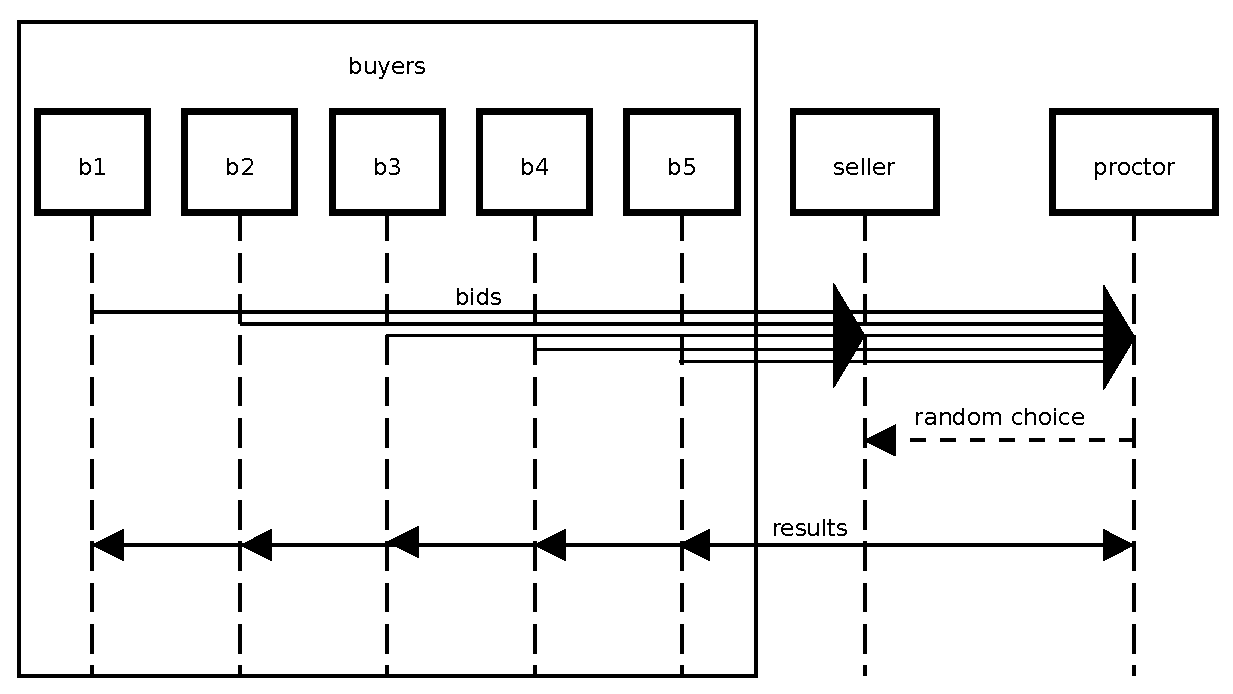
\includegraphics[width=13.5cm]{exercise.pdf}
  \end{minipage}
  \end{tabular}
  \caption{sequence diagram}
  \label{fig:usability-exercise-diagram}
    %%\Description{In the top section, twenty four lines of Haskell code using the MultiChor library, with a UML sequence diagram of that program.
%%	  }
  \end{mdframed}
\end{figure}


\end{document}
